\documentclass[]{article}
\usepackage{lmodern}
\usepackage{amssymb,amsmath}
\usepackage{ifxetex,ifluatex}
\usepackage{fixltx2e} % provides \textsubscript
\ifnum 0\ifxetex 1\fi\ifluatex 1\fi=0 % if pdftex
  \usepackage[T1]{fontenc}
  \usepackage[utf8]{inputenc}
\else % if luatex or xelatex
  \ifxetex
    \usepackage{mathspec}
    \usepackage{xltxtra,xunicode}
  \else
    \usepackage{fontspec}
  \fi
  \defaultfontfeatures{Mapping=tex-text,Scale=MatchLowercase}
  \newcommand{\euro}{€}
\fi
% use upquote if available, for straight quotes in verbatim environments
\IfFileExists{upquote.sty}{\usepackage{upquote}}{}
% use microtype if available
\IfFileExists{microtype.sty}{\usepackage{microtype}}{}
\usepackage[margin=1in]{geometry}
\usepackage{color}
\usepackage{fancyvrb}
\newcommand{\VerbBar}{|}
\newcommand{\VERB}{\Verb[commandchars=\\\{\}]}
\DefineVerbatimEnvironment{Highlighting}{Verbatim}{commandchars=\\\{\}}
% Add ',fontsize=\small' for more characters per line
\newenvironment{Shaded}{}{}
\newcommand{\AlertTok}[1]{\textcolor[rgb]{1.00,0.00,0.00}{\textbf{#1}}}
\newcommand{\AnnotationTok}[1]{\textcolor[rgb]{0.38,0.63,0.69}{\textbf{\textit{#1}}}}
\newcommand{\AttributeTok}[1]{\textcolor[rgb]{0.49,0.56,0.16}{#1}}
\newcommand{\BaseNTok}[1]{\textcolor[rgb]{0.25,0.63,0.44}{#1}}
\newcommand{\BuiltInTok}[1]{#1}
\newcommand{\CharTok}[1]{\textcolor[rgb]{0.25,0.44,0.63}{#1}}
\newcommand{\CommentTok}[1]{\textcolor[rgb]{0.38,0.63,0.69}{\textit{#1}}}
\newcommand{\CommentVarTok}[1]{\textcolor[rgb]{0.38,0.63,0.69}{\textbf{\textit{#1}}}}
\newcommand{\ConstantTok}[1]{\textcolor[rgb]{0.53,0.00,0.00}{#1}}
\newcommand{\ControlFlowTok}[1]{\textcolor[rgb]{0.00,0.44,0.13}{\textbf{#1}}}
\newcommand{\DataTypeTok}[1]{\textcolor[rgb]{0.56,0.13,0.00}{#1}}
\newcommand{\DecValTok}[1]{\textcolor[rgb]{0.25,0.63,0.44}{#1}}
\newcommand{\DocumentationTok}[1]{\textcolor[rgb]{0.73,0.13,0.13}{\textit{#1}}}
\newcommand{\ErrorTok}[1]{\textcolor[rgb]{1.00,0.00,0.00}{\textbf{#1}}}
\newcommand{\ExtensionTok}[1]{#1}
\newcommand{\FloatTok}[1]{\textcolor[rgb]{0.25,0.63,0.44}{#1}}
\newcommand{\FunctionTok}[1]{\textcolor[rgb]{0.02,0.16,0.49}{#1}}
\newcommand{\ImportTok}[1]{#1}
\newcommand{\InformationTok}[1]{\textcolor[rgb]{0.38,0.63,0.69}{\textbf{\textit{#1}}}}
\newcommand{\KeywordTok}[1]{\textcolor[rgb]{0.00,0.44,0.13}{\textbf{#1}}}
\newcommand{\NormalTok}[1]{#1}
\newcommand{\OperatorTok}[1]{\textcolor[rgb]{0.40,0.40,0.40}{#1}}
\newcommand{\OtherTok}[1]{\textcolor[rgb]{0.00,0.44,0.13}{#1}}
\newcommand{\PreprocessorTok}[1]{\textcolor[rgb]{0.74,0.48,0.00}{#1}}
\newcommand{\RegionMarkerTok}[1]{#1}
\newcommand{\SpecialCharTok}[1]{\textcolor[rgb]{0.25,0.44,0.63}{#1}}
\newcommand{\SpecialStringTok}[1]{\textcolor[rgb]{0.73,0.40,0.53}{#1}}
\newcommand{\StringTok}[1]{\textcolor[rgb]{0.25,0.44,0.63}{#1}}
\newcommand{\VariableTok}[1]{\textcolor[rgb]{0.10,0.09,0.49}{#1}}
\newcommand{\VerbatimStringTok}[1]{\textcolor[rgb]{0.25,0.44,0.63}{#1}}
\newcommand{\WarningTok}[1]{\textcolor[rgb]{0.38,0.63,0.69}{\textbf{\textit{#1}}}}
\usepackage{graphicx}
\makeatletter
\def\maxwidth{\ifdim\Gin@nat@width>\linewidth\linewidth\else\Gin@nat@width\fi}
\def\maxheight{\ifdim\Gin@nat@height>\textheight\textheight\else\Gin@nat@height\fi}
\makeatother
% Scale images if necessary, so that they will not overflow the page
% margins by default, and it is still possible to overwrite the defaults
% using explicit options in \includegraphics[width, height, ...]{}
\setkeys{Gin}{width=\maxwidth,height=\maxheight,keepaspectratio}
\ifxetex
  \usepackage[setpagesize=false, % page size defined by xetex
              unicode=false, % unicode breaks when used with xetex
              xetex]{hyperref}
\else
  \usepackage[unicode=true]{hyperref}
\fi
\hypersetup{breaklinks=true,
            bookmarks=true,
            pdfauthor={Justin Le},
            pdftitle={A Purely Functional Typed Approach to Trainable Models},
            colorlinks=true,
            citecolor=blue,
            urlcolor=blue,
            linkcolor=magenta,
            pdfborder={0 0 0}}
\urlstyle{same}  % don't use monospace font for urls
% Make links footnotes instead of hotlinks:
\renewcommand{\href}[2]{#2\footnote{\url{#1}}}
\setlength{\parindent}{0pt}
\setlength{\parskip}{6pt plus 2pt minus 1pt}
\setlength{\emergencystretch}{3em}  % prevent overfull lines
\setcounter{secnumdepth}{0}

\title{A Purely Functional Typed Approach to Trainable Models}
\author{Justin Le}

\begin{document}
\maketitle

\emph{Originally posted on
\textbf{\href{https://blog.jle.im/entry/purely-functional-typed-models.html}{in
Code}}.}

With the release of
\href{http://hackage.haskell.org/package/backprop}{backprop}, I've been
exploring the space of parameterized models of all sorts, from linear and
logistic regression and other statistical models to artificial neural networks,
feed-forward and recurrent (stateful). I wanted to see to what extent we can
really apply automatic differentiation and iterative gradient decent-based
training to all of these different models. Basically, I wanted to see how far we
can take \emph{differentiable programming} (a la
\href{https://www.facebook.com/yann.lecun/posts/10155003011462143}{Yann LeCun})
as a paradigm for writing trainable models.

I'm starting to see a picture unifying all of these models, painted in the
language of purely typed functional programming. I'm already applying these to
models I'm using in real life and in my research, and I thought I'd take some
time to put my thoughts to writing in case anyone else finds these illuminating
or useful.

As a big picture, I really believe that a purely functional typed approach to
differentiable programming is \emph{the} way to move forward in the future for
models like artificial neural networks. In this light, the drawbacks of
object-oriented and imperative approaches becomes very apparent.

I'm not the first person to attempt to build a conceptual framework for these
types of models in a purely functional typed sense --
\href{http://colah.github.io/posts/2015-09-NN-Types-FP/}{Christopher Olah's
famous post} wrote a great piece in 2015 that this post heavily builds off of,
and is definitely worth a read! We'll be taking some of his ideas and seeing how
they work in real code!

The code in this post is written in Haskell, using the
\href{http://hackage.haskell.org/package/backprop}{backprop},
\href{http://hackage.haskell.org/package/hmatrix}{hmatrix} (with
\href{http://hackage.haskell.org/package/hmatrix-backprop}{hmatrix-backprop}),
and \href{http://hackage.haskell.org/package/vector-sized}{vector-sized}
libraries.

\hypertarget{essence-of-a-model}{%
\section{Essence of a Model}\label{essence-of-a-model}}

For the purpose of this post, a \emph{parameterized model} is a function from
some input ``question'' (predictor, independent variable) to some output
``answer'' (predictand, dependent variable)

Notationally, we might write it as a function:

{[} f\_p(x) =
y{]}(https://latex.codecogs.com/png.latex?\%0Af\_p\%28x\%29\%20\%3D\%20y\%0A "
f\_p(x) = y ``)

The important thing is that, for every choice of \emph{parameterization}
\includegraphics{https://latex.codecogs.com/png.latex?p}, we get a
\emph{different function}
\includegraphics{https://latex.codecogs.com/png.latex?f_p\%28x\%29}.

For example, you might want to write a model that, when given an email, outputs
whether or not that email is spam.

The parameterization \emph{p} is some piece of data that we tweak to produce a
different \includegraphics{https://latex.codecogs.com/png.latex?f_p\%28x\%29}.
So, ``training'' (or ``learning'', or ``estimating'') a model is a process of
picking the \includegraphics{https://latex.codecogs.com/png.latex?p} that gives
the ``correct'' function
\includegraphics{https://latex.codecogs.com/png.latex?f_p\%28x\%29} --- that is,
the function that accurately predicts spam or whatever thing you are trying to
predict.

For example, for \href{https://en.wikipedia.org/wiki/Linear_regression}{linear
regression}, you are trying to ``fit'' your
\includegraphics{https://latex.codecogs.com/png.latex?\%28x\%2C\%20y\%29} data
points to some function
\includegraphics{https://latex.codecogs.com/png.latex?f\%28x\%29\%20\%3D\%20\%5Cbeta\%20\%2B\%20\%5Calpha\%20x}.
The \emph{parameters} are
\includegraphics{https://latex.codecogs.com/png.latex?\%5Calpha} and
\includegraphics{https://latex.codecogs.com/png.latex?\%5Cbeta}, the
\emph{input} is \includegraphics{https://latex.codecogs.com/png.latex?x}, and
the \emph{output} is
\includegraphics{https://latex.codecogs.com/png.latex?\%5Cbeta\%20\%2B\%20\%5Calpha\%20x}.

As it so happens, a
\includegraphics{https://latex.codecogs.com/png.latex?f_p\%28x\%29} is really
just a ``partially applied''
\includegraphics{https://latex.codecogs.com/png.latex?f\%28p\%2Cx\%29}.
Imagining that function, it has type:\footnote{Those familiar with Haskell
  idioms might recognize this type as being essentially
  \texttt{a\ -\textgreater{}\ Reader\ p\ b} (or
  \texttt{Kleisli\ (Reader\ p)\ a\ b}) which roughly represents the notion of
  ``A function from \texttt{a} to \texttt{b} with an `environment' of type
  \texttt{p}''.}

{[} f : P \textbackslash{}times A \textbackslash{}rightarrow
B{]}(https://latex.codecogs.com/png.latex?\%0Af\%20\%3A\%20P\%20\%5Ctimes\%20A\%20\%5Crightarrow\%20B\%0A
" f : P \times A \rightarrow B ``)

If we \href{https://en.wikipedia.org/wiki/Currying}{curry} this, we get the
original model representation we talked about:

{[} f : P \textbackslash{}rightarrow (A \textbackslash{}rightarrow
B){]}(https://latex.codecogs.com/png.latex?\%0Af\%20\%3A\%20P\%20\%5Crightarrow\%20\%28A\%20\%5Crightarrow\%20B\%29\%0A
" f : P \rightarrow (A \rightarrow B) ``)

\hypertarget{optimizing-models-with-observations}{%
\subsection{Optimizing Models with
Observations}\label{optimizing-models-with-observations}}

Something interesting happens if we flip the script. What if, instead of
\includegraphics{https://latex.codecogs.com/png.latex?f_p\%28x\%29}, we talked
about \includegraphics{https://latex.codecogs.com/png.latex?f_x\%28p\%29}? That
is, we fix the input and vary the parameter, and see what type of outputs we get
for the same output while we vary the parameter?

If we have an ``expected output'' for our input, then one thing we can do is
look at \includegraphics{https://latex.codecogs.com/png.latex?f_p\%28x\%29} and
see when the result is close to
\includegraphics{https://latex.codecogs.com/png.latex?y_x} (the expected output
of our model when given
\includegraphics{https://latex.codecogs.com/png.latex?x}).

In fact, we can turn this into an optimization problem by trying to pick
\includegraphics{https://latex.codecogs.com/png.latex?p} that minimizes the
difference between
\includegraphics{https://latex.codecogs.com/png.latex?f_x\%28p\%29} and
\includegraphics{https://latex.codecogs.com/png.latex?y_x}. We can say that our
model with parameter \includegraphics{https://latex.codecogs.com/png.latex?p}
predicts \includegraphics{https://latex.codecogs.com/png.latex?y_x} the best
when we minimize:

{[} (f\_x(p) -
y\_x)\^{}2{]}(https://latex.codecogs.com/png.latex?\%0A\%28f\_x\%28p\%29\%20-\%20y\_x\%29\%5E2\%0A
" (f\_x(p) - y\_x)\^{}2 ``)

If we minimize the squared error between the result of picking the parameter and
the expected result, we find the best parameters for that given input!

In general, picking the best parameter for the model involves picking the
\includegraphics{https://latex.codecogs.com/png.latex?p} that minimizes the
relationship

{[} \textbackslash{}text\{loss\}(y\_x,
f\_x(p)){]}(https://latex.codecogs.com/png.latex?\%0A\%5Ctext\%7Bloss\%7D\%28y\_x\%2C\%20f\_x\%28p\%29\%29\%0A
" \text{loss}(y\_x, f\_x(p)) ``)

Where
\includegraphics{https://latex.codecogs.com/png.latex?\%5Ctext\%7Bloss\%7D\%20\%3A\%20B\%20\%5Ctimes\%20B\%20\%5Crightarrow\%20\%5Cmathbb\%7BR\%7D}
gives a measure of ``how badly'' the model result differs from the expected
target. Common loss functions include squared error, cross-entropy, etc.

This gives us a supervised way to train any model: if we have enough
observations
(\includegraphics{https://latex.codecogs.com/png.latex?\%28x\%2C\%20y_x\%29}
pairs) we can just pick a
\includegraphics{https://latex.codecogs.com/png.latex?p} that does its best to
make the loss between all observations as small as possible.

\hypertarget{stochastic-gradient-descent}{%
\subsection{Stochastic Gradient Descent}\label{stochastic-gradient-descent}}

If our model is a \emph{differentiable function}, then we have a nice tool we
can use: \emph{stochastic gradient descent} (SGD).

That is, we can always calculate the \emph{gradient} of the loss function with
respect to our parameters. This gives us the direction we can ``nudge'' our
parameters to make the loss bigger or smaller.

That is, if we get the gradient of the loss with respect to
\includegraphics{https://latex.codecogs.com/png.latex?p}:

{[} \textbackslash{}nabla\_p \textbackslash{}text\{loss\}(f\_x(p),
y\_x){]}(https://latex.codecogs.com/png.latex?\%0A\%5Cnabla\_p\%20\%5Ctext\%7Bloss\%7D\%28f\_x\%28p\%29\%2C\%20y\_x\%29\%0A
" \nabla\_p \text{loss}(f\_x(p), y\_x) ``)

We now have a nice way to ``train'' our model:

\begin{enumerate}
\def\labelenumi{\arabic{enumi}.}
\tightlist
\item
  Start with an initial guess at the parameter
\item
  Look at a random
  \includegraphics{https://latex.codecogs.com/png.latex?\%28x\%2C\%20y_x\%29}
  observation pair.
\item
  Compute the gradient
  \includegraphics{https://latex.codecogs.com/png.latex?\%5Cnabla_p\%20\%5Ctext\%7Bloss\%7D\%28f_x\%28p\%29\%2C\%20y_x\%29}
  of our current \includegraphics{https://latex.codecogs.com/png.latex?p}, which
  tells us a direction we can ``nudge''
  \includegraphics{https://latex.codecogs.com/png.latex?p} in to make the loss
  smaller.
\item
  Nudge \includegraphics{https://latex.codecogs.com/png.latex?p} in that
  direction
\item
  Repeat from \#2 until satisfied
\end{enumerate}

With every new observation, we see how we can nudge the parameter to make the
model more accurate, and then we perform that nudge.

\hypertarget{functional-implementation}{%
\section{Functional Implementation}\label{functional-implementation}}

This naturally lends itself well to a functional implementation. That's because,
in this light, a model is nothing more than a function. And a model that is
trainable using SGD is simply a differentiable function.

Using the \emph{\href{http://hackage.haskell.org/package/backprop}{backprop}}
library, we can easily write functions to be differentiable.

Let's write the type of our models. A model from type \texttt{a} to type
\texttt{b} with parameter \texttt{p} can be written as

\begin{Shaded}
\begin{Highlighting}[]
\KeywordTok{type} \DataTypeTok{Model}\NormalTok{ p a b }\FunctionTok{=}\NormalTok{ p }\OtherTok{->}\NormalTok{ a }\OtherTok{->}\NormalTok{ b}
\end{Highlighting}
\end{Shaded}

Not normally differentiable, but we can make it a differentiable function by
having it work with \texttt{BVar\ z\ p} and \texttt{BVar\ z\ a} (\texttt{BVar}s
containing those values) instead:

\begin{Shaded}
\begin{Highlighting}[]
\CommentTok{-- source: https://github.com/mstksg/inCode/tree/master/code-samples/functional-models/model.hs#L48-L49}

\KeywordTok{type} \DataTypeTok{Model}\NormalTok{ p a b }\FunctionTok{=}\NormalTok{ forall z}\FunctionTok{.} \DataTypeTok{Reifies}\NormalTok{ z }\DataTypeTok{W}
                \OtherTok{=>} \DataTypeTok{BVar}\NormalTok{ z p }\OtherTok{->} \DataTypeTok{BVar}\NormalTok{ z a }\OtherTok{->} \DataTypeTok{BVar}\NormalTok{ z b}
\end{Highlighting}
\end{Shaded}

We can write a simple linear regression model:

{[} f\_\{\textbackslash{}alpha, \textbackslash{}beta\}(x) = \textbackslash{}beta
x +
\textbackslash{}alpha{]}(https://latex.codecogs.com/png.latex?\%0Af\_\%7B\%5Calpha\%2C\%20\%5Cbeta\%7D\%28x\%29\%20\%3D\%20\%5Cbeta\%20x\%20\%2B\%20\%5Calpha\%0A
" f\_\{\alpha, \beta\}(x) = \beta x + \alpha ``)

\begin{Shaded}
\begin{Highlighting}[]
\CommentTok{-- source: https://github.com/mstksg/inCode/tree/master/code-samples/functional-models/model.hs#L44-L55}

\KeywordTok{data}\NormalTok{ a }\FunctionTok{:&}\NormalTok{ b }\FunctionTok{=} \FunctionTok{!}\NormalTok{a }\FunctionTok{:&} \FunctionTok{!}\NormalTok{b}

\OtherTok{linReg ::} \DataTypeTok{Model}\NormalTok{ (}\DataTypeTok{Double} \FunctionTok{:&} \DataTypeTok{Double}\NormalTok{) }\DataTypeTok{Double} \DataTypeTok{Double}
\NormalTok{linReg ab x }\FunctionTok{=}\NormalTok{ b }\FunctionTok{*}\NormalTok{ x }\FunctionTok{+}\NormalTok{ a}
  \KeywordTok{where}
\NormalTok{    a }\FunctionTok{=}\NormalTok{ ab }\FunctionTok{^^.}\NormalTok{ t1}
\NormalTok{    b }\FunctionTok{=}\NormalTok{ ab }\FunctionTok{^^.}\NormalTok{ t2}
\end{Highlighting}
\end{Shaded}

(First we define a custom tuple data type \texttt{:\&}; backprop works with
normal tuples, but using a custom tuple with a \texttt{Num} instance will come
in handy later for training models)

Here \texttt{Double\ :\&\ Double} is a tuple of two \texttt{Double}s, which
contains the parameters (\texttt{a} and \texttt{b}). We extract the first item
using \texttt{\^{}\^{}.\ t1} and the second item with \texttt{\^{}\^{}.\ t2}
(\texttt{t1} and \texttt{t2} being lenses defined for the tuple fields), and
then talk about the actual function, whose result is \texttt{b\ *\ x\ +\ a}.
Note that, because \texttt{BVar}s have a \texttt{Num} instance, we can use all
our normal numeric operators, and the results are still differentiable.

We can \emph{run} \texttt{linReg} using \texttt{evalBP2}:

\begin{Shaded}
\begin{Highlighting}[]
\NormalTok{ghci}\FunctionTok{>}\NormalTok{ evalBP2 linReg (}\FloatTok{0.3} \FunctionTok{:&}\NormalTok{ (}\FunctionTok{-}\FloatTok{0.1}\NormalTok{)) }\DecValTok{5}
\FunctionTok{-}\FloatTok{0.2}        \CommentTok{-- (-0.1) * 5 + 0.3}
\end{Highlighting}
\end{Shaded}

But the neat thing is that we can also get the gradient of the parameters, too,
if we identify a loss function:\footnote{Note that this is only sound as a loss
  function for a single ``scalar value'', like \texttt{Double} or a one-vector.
  In general, we'd have this take a loss function as a parameter.}

{[} \textbackslash{}nabla\_p (f(p, x) -
y\_x)\^{}2{]}(https://latex.codecogs.com/png.latex?\%0A\%5Cnabla\_p\%20\%28f\%28p\%2C\%20x\%29\%20-\%20y\_x\%29\%5E2\%0A
" \nabla\_p (f(p, x) - y\_x)\^{}2 ``)

\begin{Shaded}
\begin{Highlighting}[]
\CommentTok{-- source: https://github.com/mstksg/inCode/tree/master/code-samples/functional-models/model.hs#L57-L65}

\NormalTok{squaredErrorGrad}
\OtherTok{    ::}\NormalTok{ (}\DataTypeTok{Backprop}\NormalTok{ p, }\DataTypeTok{Backprop}\NormalTok{ b, }\DataTypeTok{Num}\NormalTok{ b)}
    \OtherTok{=>} \DataTypeTok{Model}\NormalTok{ p a b      }\CommentTok{-- ^ Model}
    \OtherTok{->}\NormalTok{ a                }\CommentTok{-- ^ Observed input}
    \OtherTok{->}\NormalTok{ b                }\CommentTok{-- ^ Observed output}
    \OtherTok{->}\NormalTok{ p                }\CommentTok{-- ^ Parameter guess}
    \OtherTok{->}\NormalTok{ p                }\CommentTok{-- ^ Gradient}
\NormalTok{squaredErrorGrad f x targ }\FunctionTok{=}\NormalTok{ gradBP }\FunctionTok{$}\NormalTok{ \textbackslash{}p }\OtherTok{->}
\NormalTok{    (f p (auto x) }\FunctionTok{-}\NormalTok{ auto targ) }\FunctionTok{^} \DecValTok{2}
\end{Highlighting}
\end{Shaded}

We use \texttt{auto\ ::\ a\ -\textgreater{}\ BVar\ z\ a}, to lift a normal value
to a \texttt{BVar} holding that value, since our model \texttt{f} takes
\texttt{BVar}s.

And finally, we can train it using stochastic gradient descent, with just a
simple fold over all observations:

\begin{Shaded}
\begin{Highlighting}[]
\CommentTok{-- source: https://github.com/mstksg/inCode/tree/master/code-samples/functional-models/model.hs#L67-L73}

\NormalTok{trainModel}
\OtherTok{    ::}\NormalTok{ (}\DataTypeTok{Fractional}\NormalTok{ p, }\DataTypeTok{Backprop}\NormalTok{ p, }\DataTypeTok{Num}\NormalTok{ b, }\DataTypeTok{Backprop}\NormalTok{ b)}
    \OtherTok{=>} \DataTypeTok{Model}\NormalTok{ p a b      }\CommentTok{-- ^ model to train}
    \OtherTok{->}\NormalTok{ p                }\CommentTok{-- ^ initial parameter guess}
    \OtherTok{->}\NormalTok{ [(a,b)]          }\CommentTok{-- ^ list of observations}
    \OtherTok{->}\NormalTok{ p                }\CommentTok{-- ^ updated parameter guess}
\NormalTok{trainModel f }\FunctionTok{=}\NormalTok{ foldl' }\FunctionTok{$}\NormalTok{ \textbackslash{}p (x,y) }\OtherTok{->}\NormalTok{ p }\FunctionTok{-} \FloatTok{0.1} \FunctionTok{*}\NormalTok{ squaredErrorGrad f x y p}
\end{Highlighting}
\end{Shaded}

For convenience, we can define a \texttt{Random} instance for our tuple type
using the \emph{\href{http://hackage.haskell.org/package/random}{random}}
library and make a wrapper that uses \texttt{IO} to generate a random initial
parameter:

\begin{Shaded}
\begin{Highlighting}[]
\CommentTok{-- source: https://github.com/mstksg/inCode/tree/master/code-samples/functional-models/model.hs#L75-L82}

\NormalTok{trainModelIO}
\OtherTok{    ::}\NormalTok{ (}\DataTypeTok{Fractional}\NormalTok{ p, }\DataTypeTok{Backprop}\NormalTok{ p, }\DataTypeTok{Num}\NormalTok{ b, }\DataTypeTok{Backprop}\NormalTok{ b, }\DataTypeTok{Random}\NormalTok{ p)}
    \OtherTok{=>} \DataTypeTok{Model}\NormalTok{ p a b      }\CommentTok{-- ^ model to train}
    \OtherTok{->}\NormalTok{ [(a,b)]          }\CommentTok{-- ^ list of observations}
    \OtherTok{->} \DataTypeTok{IO}\NormalTok{ p             }\CommentTok{-- ^ parameter guess}
\NormalTok{trainModelIO m xs }\FunctionTok{=} \KeywordTok{do}
\NormalTok{    p0 }\OtherTok{<-}\NormalTok{ (}\FunctionTok{/} \DecValTok{10}\NormalTok{) }\FunctionTok{.}\NormalTok{ subtract }\FloatTok{0.5} \FunctionTok{<$>}\NormalTok{ randomIO}
\NormalTok{    return }\FunctionTok{$}\NormalTok{ trainModel m p0 xs}
\end{Highlighting}
\end{Shaded}

Let's train our linear regression model to fit the points \texttt{(1,1)},
\texttt{(2,3)}, \texttt{(3,5)}, \texttt{(4,7)}, and \texttt{(5,9)}! This should
follow
\includegraphics{https://latex.codecogs.com/png.latex?f\%28x\%29\%20\%3D\%202\%20x\%20-\%201},
or
\includegraphics{https://latex.codecogs.com/png.latex?\%5Calpha\%20\%3D\%20-1\%2C\%5C\%2C\%20\%5Cbeta\%20\%3D\%202}:

\begin{Shaded}
\begin{Highlighting}[]
\NormalTok{ghci}\FunctionTok{>}\NormalTok{ samps }\FunctionTok{=}\NormalTok{ [(}\DecValTok{1}\NormalTok{,}\DecValTok{1}\NormalTok{),(}\DecValTok{2}\NormalTok{,}\DecValTok{3}\NormalTok{),(}\DecValTok{3}\NormalTok{,}\DecValTok{5}\NormalTok{),(}\DecValTok{4}\NormalTok{,}\DecValTok{7}\NormalTok{),(}\DecValTok{5}\NormalTok{,}\DecValTok{9}\NormalTok{)]}
\NormalTok{ghci}\FunctionTok{>}\NormalTok{ trainModelIO linReg }\FunctionTok{$}\NormalTok{ take }\DecValTok{5000}\NormalTok{ (cycle samps)}
\NormalTok{(}\FunctionTok{-}\FloatTok{1.0000000000000024}\NormalTok{) }\FunctionTok{:&} \FloatTok{2.0000000000000036}
\CommentTok{-- roughly:}
\NormalTok{(}\FunctionTok{-}\FloatTok{1.0}\NormalTok{) }\FunctionTok{:&} \FloatTok{2.0}
\end{Highlighting}
\end{Shaded}

Neat! After going through all of those observations a thousand times, the model
nudges itself all the way to the right parameters to fit our model!

The important takeaway is that all we specified was the \emph{function} of the
model itself. The training part all follows automatically.

\hypertarget{feed-forward-neural-network}{%
\subsection{Feed-forward Neural Network}\label{feed-forward-neural-network}}

Here's another example: a feed-forward neural network.

We can start with a single layer. The model here will also take two parameters
(a weight matrix and a bias vector), take in a vector, and output a vector.

\begin{Shaded}
\begin{Highlighting}[]
\KeywordTok{import} \DataTypeTok{Numeric.LinearAlgebra.Static.Backprop}
\CommentTok{-- source: https://github.com/mstksg/inCode/tree/master/code-samples/functional-models/model.hs#L89-L106}

\OtherTok{logistic ::} \DataTypeTok{Floating}\NormalTok{ a }\OtherTok{=>}\NormalTok{ a }\OtherTok{->}\NormalTok{ a}
\NormalTok{logistic x }\FunctionTok{=} \DecValTok{1} \FunctionTok{/}\NormalTok{ (}\DecValTok{1} \FunctionTok{+}\NormalTok{ exp (}\FunctionTok{-}\NormalTok{x))}

\NormalTok{feedForwardLog}
\OtherTok{    ::}\NormalTok{ (}\DataTypeTok{KnownNat}\NormalTok{ i, }\DataTypeTok{KnownNat}\NormalTok{ o)}
    \OtherTok{=>} \DataTypeTok{Model}\NormalTok{ (}\DataTypeTok{L}\NormalTok{ o i }\FunctionTok{:&} \DataTypeTok{R}\NormalTok{ o) (}\DataTypeTok{R}\NormalTok{ i) (}\DataTypeTok{R}\NormalTok{ o)}
\NormalTok{feedForwardLog wb x }\FunctionTok{=}\NormalTok{ logistic (w }\FunctionTok{#>}\NormalTok{ x }\FunctionTok{+}\NormalTok{ b)}
  \KeywordTok{where}
\NormalTok{    w }\FunctionTok{=}\NormalTok{ wb }\FunctionTok{^^.}\NormalTok{ t1}
\NormalTok{    b }\FunctionTok{=}\NormalTok{ wb }\FunctionTok{^^.}\NormalTok{ t2}
\end{Highlighting}
\end{Shaded}

Here we use the \texttt{L\ n\ m} (an n-by-m matrix) and \texttt{R\ n} (an
n-vector) types from the \emph{hmatrix} library, and \texttt{\#\textgreater{}}
for backprop-aware matrix-vector multiplication.

Let's try training a model to learn the simple
\href{https://en.wikipedia.org/wiki/Logical_conjunction}{logical ``AND''}:

\begin{Shaded}
\begin{Highlighting}[]
\NormalTok{ghci}\FunctionTok{>} \KeywordTok{import} \KeywordTok{qualified} \DataTypeTok{Numeric.LinearAlgebra.Static} \KeywordTok{as} \DataTypeTok{H}
\NormalTok{ghci}\FunctionTok{>}\NormalTok{ samps }\FunctionTok{=}\NormalTok{ [(H.vec2 }\DecValTok{0} \DecValTok{0}\NormalTok{, }\DecValTok{0}\NormalTok{), (H.vec2 }\DecValTok{1} \DecValTok{0}\NormalTok{, }\DecValTok{0}\NormalTok{), (H.vec2 }\DecValTok{0} \DecValTok{1}\NormalTok{, }\DecValTok{0}\NormalTok{), (H.vec2 }\DecValTok{1} \DecValTok{1}\NormalTok{, }\DecValTok{1}\NormalTok{)]}
\NormalTok{ghci}\FunctionTok{>}\NormalTok{ trained }\OtherTok{<-}\NormalTok{ trainModelIO feedForwardLog }\FunctionTok{$}\NormalTok{ take }\DecValTok{10000}\NormalTok{ (cycle samps)}
\end{Highlighting}
\end{Shaded}

We have our trained parameters! Let's see if they actually model ``AND''?

\begin{Shaded}
\begin{Highlighting}[]
\NormalTok{ghci}\FunctionTok{>}\NormalTok{ evalBP2 feedForwardLog trained (H.vec2 }\DecValTok{0} \DecValTok{0}\NormalTok{)}
\NormalTok{(}\FloatTok{7.468471910660985e-5}\OtherTok{ ::} \DataTypeTok{R} \DecValTok{1}\NormalTok{)       }\CommentTok{-- 0.0}
\NormalTok{ghci}\FunctionTok{>}\NormalTok{ evalBP2 feedForwardLog trained (H.vec2 }\DecValTok{1} \DecValTok{0}\NormalTok{)}
\NormalTok{(}\FloatTok{3.816205998697482e-2}\OtherTok{ ::} \DataTypeTok{R} \DecValTok{1}\NormalTok{)       }\CommentTok{-- 0.0}
\NormalTok{ghci}\FunctionTok{>}\NormalTok{ evalBP2 feedForwardLog trained (H.vec2 }\DecValTok{0} \DecValTok{1}\NormalTok{)}
\NormalTok{(}\FloatTok{3.817490115313559e-2}\OtherTok{ ::} \DataTypeTok{R} \DecValTok{1}\NormalTok{)       }\CommentTok{-- 0.0}
\NormalTok{ghci}\FunctionTok{>}\NormalTok{ evalBP2 feedForwardLog trained (H.vec2 }\DecValTok{1} \DecValTok{1}\NormalTok{)}
\NormalTok{(}\FloatTok{0.9547178031665701}\OtherTok{ ::} \DataTypeTok{R} \DecValTok{1}\NormalTok{)         }\CommentTok{-- 1.0}
\end{Highlighting}
\end{Shaded}

Close enough for me!

If we inspect the arrived-at parameters, we can see what makes the network tick:

\begin{Shaded}
\begin{Highlighting}[]
\NormalTok{ghci}\FunctionTok{>}\NormalTok{ trained}
\NormalTok{(matrix}
\NormalTok{ [ }\FloatTok{4.652034474187562}\NormalTok{, }\FloatTok{4.65355702367007}\NormalTok{ ]}\OtherTok{ ::} \DataTypeTok{L} \DecValTok{1} \DecValTok{2}\NormalTok{) }\FunctionTok{:&}\NormalTok{ (}\FunctionTok{-}\FloatTok{7.073724083776028}\OtherTok{ ::} \DataTypeTok{R} \DecValTok{1}\NormalTok{)}
\end{Highlighting}
\end{Shaded}

It seems like there is a heavy negative bias, and that each of the inputs makes
some contribution that is slightly more than half of the negative bias; the end
goal is that one of the inputs alone makes no dent, but only if both inputs are
``on'', the output can overcome the negative bias.

The network was able to arrive that this configuration just by exploring the
gradient of our differentiable function!

\hypertarget{functional-composition}{%
\subsection{Functional composition}\label{functional-composition}}

Because our functions are simply just \emph{normal functions}, we can create
new, complex models from simpler ones using just functional composition.

For example, we can map the result of a model to create a new model. Here, we
compose \texttt{linReg\ ab} (linear regression with parameter \texttt{ab}) with
the logistic function to create a
\emph{\href{https://en.wikipedia.org/wiki/Logistic_regression}{logistic
regression}} model.

\begin{Shaded}
\begin{Highlighting}[]
\CommentTok{-- source: https://github.com/mstksg/inCode/tree/master/code-samples/functional-models/model.hs#L120-L121}

\OtherTok{logReg ::} \DataTypeTok{Model}\NormalTok{ (}\DataTypeTok{Double} \FunctionTok{:&} \DataTypeTok{Double}\NormalTok{) }\DataTypeTok{Double} \DataTypeTok{Double}
\NormalTok{logReg ab }\FunctionTok{=}\NormalTok{ logistic }\FunctionTok{.}\NormalTok{ linReg ab}
\end{Highlighting}
\end{Shaded}

We could have even written our \texttt{feedForwardLog} without its activation
function:

\begin{Shaded}
\begin{Highlighting}[]
\CommentTok{-- source: https://github.com/mstksg/inCode/tree/master/code-samples/functional-models/model.hs#L92-L98}

\NormalTok{feedForward}
\OtherTok{    ::}\NormalTok{ (}\DataTypeTok{KnownNat}\NormalTok{ i, }\DataTypeTok{KnownNat}\NormalTok{ o)}
    \OtherTok{=>} \DataTypeTok{Model}\NormalTok{ (}\DataTypeTok{L}\NormalTok{ o i }\FunctionTok{:&} \DataTypeTok{R}\NormalTok{ o) (}\DataTypeTok{R}\NormalTok{ i) (}\DataTypeTok{R}\NormalTok{ o)}
\NormalTok{feedForward wb x }\FunctionTok{=}\NormalTok{ w }\FunctionTok{#>}\NormalTok{ x }\FunctionTok{+}\NormalTok{ b}
  \KeywordTok{where}
\NormalTok{    w }\FunctionTok{=}\NormalTok{ wb }\FunctionTok{^^.}\NormalTok{ t1}
\NormalTok{    b }\FunctionTok{=}\NormalTok{ wb }\FunctionTok{^^.}\NormalTok{ t2}
\end{Highlighting}
\end{Shaded}

And now we can swap out activation functions using simple function composition:

\begin{Shaded}
\begin{Highlighting}[]
\CommentTok{-- source: https://github.com/mstksg/inCode/tree/master/code-samples/functional-models/model.hs#L123-L126}

\NormalTok{feedForwardLog'}
\OtherTok{    ::}\NormalTok{ (}\DataTypeTok{KnownNat}\NormalTok{ i, }\DataTypeTok{KnownNat}\NormalTok{ o)}
    \OtherTok{=>} \DataTypeTok{Model}\NormalTok{ (}\DataTypeTok{L}\NormalTok{ o i }\FunctionTok{:&} \DataTypeTok{R}\NormalTok{ o) (}\DataTypeTok{R}\NormalTok{ i) (}\DataTypeTok{R}\NormalTok{ o)}
\NormalTok{feedForwardLog' wb }\FunctionTok{=}\NormalTok{ logistic }\FunctionTok{.}\NormalTok{ feedForward wb}
\end{Highlighting}
\end{Shaded}

Maybe even a \href{https://en.wikipedia.org/wiki/Softmax_function}{softmax}
classifier!

\begin{Shaded}
\begin{Highlighting}[]
\CommentTok{-- source: https://github.com/mstksg/inCode/tree/master/code-samples/functional-models/model.hs#L128-L136}

\OtherTok{softMax ::}\NormalTok{ (}\DataTypeTok{Reifies}\NormalTok{ z }\DataTypeTok{W}\NormalTok{, }\DataTypeTok{KnownNat}\NormalTok{ n) }\OtherTok{=>} \DataTypeTok{BVar}\NormalTok{ z (}\DataTypeTok{R}\NormalTok{ n) }\OtherTok{->} \DataTypeTok{BVar}\NormalTok{ z (}\DataTypeTok{R}\NormalTok{ n)}
\NormalTok{softMax x }\FunctionTok{=}\NormalTok{ konst (}\DecValTok{1} \FunctionTok{/}\NormalTok{ sumElements expx) }\FunctionTok{*}\NormalTok{ expx}
  \KeywordTok{where}
\NormalTok{    expx }\FunctionTok{=}\NormalTok{ exp x}

\NormalTok{feedForwardSoftMax}
\OtherTok{    ::}\NormalTok{ (}\DataTypeTok{KnownNat}\NormalTok{ i, }\DataTypeTok{KnownNat}\NormalTok{ o)}
    \OtherTok{=>} \DataTypeTok{Model}\NormalTok{ (}\DataTypeTok{L}\NormalTok{ o i }\FunctionTok{:&} \DataTypeTok{R}\NormalTok{ o) (}\DataTypeTok{R}\NormalTok{ i) (}\DataTypeTok{R}\NormalTok{ o)}
\NormalTok{feedForwardSoftMax wb }\FunctionTok{=}\NormalTok{ logistic }\FunctionTok{.}\NormalTok{ feedForward wb}
\end{Highlighting}
\end{Shaded}

We can even write a function to \emph{compose} two models, keeping their two
original parameters separate:

\begin{Shaded}
\begin{Highlighting}[]
\CommentTok{-- source: https://github.com/mstksg/inCode/tree/master/code-samples/functional-models/model.hs#L138-L147}

\NormalTok{(}\FunctionTok{<~}\NormalTok{)}
\OtherTok{    ::}\NormalTok{ (}\DataTypeTok{Backprop}\NormalTok{ p, }\DataTypeTok{Backprop}\NormalTok{ q)}
    \OtherTok{=>} \DataTypeTok{Model}\NormalTok{  p       b c}
    \OtherTok{->} \DataTypeTok{Model}\NormalTok{       q  a b}
    \OtherTok{->} \DataTypeTok{Model}\NormalTok{ (p }\FunctionTok{:&}\NormalTok{ q) a c}
\NormalTok{(f }\FunctionTok{<~}\NormalTok{ g) pq }\FunctionTok{=}\NormalTok{ f p }\FunctionTok{.}\NormalTok{ g q}
  \KeywordTok{where}
\NormalTok{    p }\FunctionTok{=}\NormalTok{ pq }\FunctionTok{^^.}\NormalTok{ t1}
\NormalTok{    q }\FunctionTok{=}\NormalTok{ pq }\FunctionTok{^^.}\NormalTok{ t2}
\KeywordTok{infixr} \DecValTok{8} \FunctionTok{<~}
\end{Highlighting}
\end{Shaded}

And now we have a way to chain models! Maybe even make a multiple-layer neural
network? Let's see if we can get a two-layer model to learn
\href{https://en.wikipedia.org/wiki/Exclusive_or}{XOR}!

Our model is two feed-forward layers with logistic activation functions, with 4
hidden layer units:

\begin{Shaded}
\begin{Highlighting}[]
\NormalTok{ghci}\FunctionTok{>}\NormalTok{ twoLayer }\FunctionTok{=}\NormalTok{ feedForwardLog' }\FunctionTok{@}\DecValTok{4} \FunctionTok{@}\DecValTok{1} \FunctionTok{<~}\NormalTok{ feedForwardLog' }\FunctionTok{@}\DecValTok{2} \FunctionTok{@}\DecValTok{4}
\end{Highlighting}
\end{Shaded}

Note we use type application syntax (the \texttt{@}) to specify the input/output
dimensions of \texttt{feedForwardLog\textquotesingle{}}; when we write
\texttt{feedForwardLog\textquotesingle{}\ @4\ @1}, it means to set the
\texttt{i} type variable to \texttt{4} and the \texttt{o} type variable to
\texttt{1}.

We can train it on sample points:

\begin{Shaded}
\begin{Highlighting}[]
\NormalTok{ghci}\FunctionTok{>}\NormalTok{ samps }\FunctionTok{=}\NormalTok{ [(H.vec2 }\DecValTok{0} \DecValTok{0}\NormalTok{, }\DecValTok{0}\NormalTok{), (H.vec2 }\DecValTok{1} \DecValTok{0}\NormalTok{, }\DecValTok{1}\NormalTok{), (H.vec2 }\DecValTok{0} \DecValTok{1}\NormalTok{, }\DecValTok{1}\NormalTok{), (H.vec2 }\DecValTok{1} \DecValTok{1}\NormalTok{, }\DecValTok{1}\NormalTok{)]}
\NormalTok{ghci}\FunctionTok{>}\NormalTok{ trained }\OtherTok{<-}\NormalTok{ trainModelIO twoLayer }\FunctionTok{$}\NormalTok{ take }\DecValTok{10000}\NormalTok{ (cycle samps)}
\end{Highlighting}
\end{Shaded}

Trained. Now, does it model ``XOR''?

\begin{Shaded}
\begin{Highlighting}[]
\NormalTok{ghci}\FunctionTok{>}\NormalTok{ evalBP2 twoLayer trained (H.vec2 }\DecValTok{0} \DecValTok{0}\NormalTok{)}
\NormalTok{(}\FloatTok{3.0812844350410647e-2}\OtherTok{ ::} \DataTypeTok{R} \DecValTok{1}\NormalTok{)          }\CommentTok{-- 0.0}
\NormalTok{ghci}\FunctionTok{>}\NormalTok{ evalBP2 twoLayer trained (H.vec2 }\DecValTok{1} \DecValTok{0}\NormalTok{)}
\NormalTok{(}\FloatTok{0.959153369985914}\OtherTok{ ::} \DataTypeTok{R} \DecValTok{1}\NormalTok{)              }\CommentTok{-- 1.0}
\NormalTok{ghci}\FunctionTok{>}\NormalTok{ evalBP2 twoLayer trained (H.vec2 }\DecValTok{0} \DecValTok{1}\NormalTok{)}
\NormalTok{(}\FloatTok{0.9834757090696419}\OtherTok{ ::} \DataTypeTok{R} \DecValTok{1}\NormalTok{)             }\CommentTok{-- 1.0}
\NormalTok{ghci}\FunctionTok{>}\NormalTok{ evalBP2 twoLayer trained (H.vec2 }\DecValTok{1} \DecValTok{1}\NormalTok{)}
\NormalTok{(}\FloatTok{3.6846467867668035e-2}\OtherTok{ ::} \DataTypeTok{R} \DecValTok{1}\NormalTok{)          }\CommentTok{-- 0.0}
\end{Highlighting}
\end{Shaded}

Not bad!

\hypertarget{theyre-just-functions}{%
\subsection{They're Just Functions}\label{theyre-just-functions}}

We just built a working neural network using normal function composition and
simple combinators. No need for any objects or mutability or fancy explicit
graphs. Just pure, typed functions! Why would you ever bring anything imperative
into this?

You can build a lot with just these tools alone. By using primitive models and
the various combinators, you can create autoencoders, nonlinear regressions,
convolutional neural networks, multi-layered neural networks\ldots{}you can
create complex ``graphs'' of networks that fork and re-combine with themselves.

The nice thing is that these are all just regular (Rank-2) functions,
so\ldots{}you have two models? Just compose their functions like normal
functions!

It is tempting to look at something like

\begin{Shaded}
\begin{Highlighting}[]
\NormalTok{feedForwardLog }\FunctionTok{@}\DecValTok{4} \FunctionTok{@}\DecValTok{1} \FunctionTok{<~}\NormalTok{ feedForwardLog }\FunctionTok{@}\DecValTok{2} \FunctionTok{@}\DecValTok{4}
\end{Highlighting}
\end{Shaded}

and think of it as some sort of abstract, opaque data type with magic inside.
After all, ``layers'' are ``data'', right? But, at the end of the day, it's all
just:

\begin{Shaded}
\begin{Highlighting}[]
\NormalTok{\textbackslash{}pq }\OtherTok{->}\NormalTok{ feedForwardLog }\FunctionTok{@}\DecValTok{4} \FunctionTok{@}\DecValTok{1}\NormalTok{ (pq }\FunctionTok{^^.}\NormalTok{ t1) }\FunctionTok{.}\NormalTok{ feedForwardLog }\FunctionTok{@}\DecValTok{2} \FunctionTok{@}\DecValTok{4}\NormalTok{ (pq }\FunctionTok{^^.}\NormalTok{ t2)}
\end{Highlighting}
\end{Shaded}

Just normal function composition -- we're really just defining the
\emph{function} itself, and \emph{backprop} turns that function into a trainable
model.

In the past I've talked about
\href{https://blog.jle.im/entry/practical-dependent-types-in-haskell-1.html}{layers
as data}, and neural network libraries like
\href{http://hackage.haskell.org/package/grenade-0.1.0}{grenade} let you
manipulate neural network layers in a composable way. My previous attempts at
neural networks like \href{https://github.com/mstksg/tensor-ops}{tensor-ops}
also force a similar structure of composition of data types. However, I feel
this is a bit limiting.

You are forced to ``compose'' your layers in only the ways that the API of the
data type gives you. You have to use the data type's ``function composition''
functions, or its special ``mapping'' functions\ldots{}and for weird things like
forking compositions like
\texttt{\textbackslash{}f\ g\ h\ x\ -\textgreater{}\ f\ (g\ x)\ (h\ x)} you have
to learn how the data type offers such an API.

However, such a crazy composition here is ``trivial'' -- it's all just normal
functions, so you can just literally write out code like
\texttt{\textbackslash{}f\ g\ h\ x\ -\textgreater{}\ f\ (g\ x)\ (h\ x)} (or
something very close). You don't have to learn any rules of special ``layer''
data types. At the heart of it all, your model is \emph{just a function}. And,
with differentiable programming, it's a \emph{trainable function}.

\hypertarget{time-series-models}{%
\section{Time Series Models}\label{time-series-models}}

Not all models are ``question and answer'' models, however -- some models
represent a time series. As a generalization, we can talk about time series
models as:

{[} f\_p(x,t) =
y{]}(https://latex.codecogs.com/png.latex?\%0Af\_p\%28x\%2Ct\%29\%20\%3D\%20y\%0A
" f\_p(x,t) = y ``)

Which says, given an input and a time, return an output based on both. The point
of this is to let us have recurrent relationships, like for autoregressive
models:

{[} \textbackslash{}text\{AR\}\_\{\textbackslash{}phi\_1,
\textbackslash{}phi\_2, \textbackslash{}ldots\}(x,t) =
\textbackslash{}epsilon\_t + \textbackslash{}phi\_1
\textbackslash{}text\{AR\}\_\{\textbackslash{}phi\_1, \textbackslash{}phi\_2,
\textbackslash{}ldots\}(x, t-1) + \textbackslash{}phi\_2
\textbackslash{}text\{AR\}\_\{\textbackslash{}phi\_1, \textbackslash{}phi\_2,
\textbackslash{}ldots\}(x, t-2) +
\textbackslash{}ldots{]}(https://latex.codecogs.com/png.latex?\%0A\%5Ctext\%7BAR\%7D\_\%7B\%5Cphi\_1\%2C\%20\%5Cphi\_2\%2C\%20\%5Cldots\%7D\%28x\%2Ct\%29\%0A\%20\%20\%3D\%20\%5Cepsilon\_t\%20\%2B\%20\%5Cphi\_1\%20\%5Ctext\%7BAR\%7D\_\%7B\%5Cphi\_1\%2C\%20\%5Cphi\_2\%2C\%20\%5Cldots\%7D\%28x\%2C\%20t-1\%29\%0A\%20\%20\%2B\%20\%5Cphi\_2\%20\%5Ctext\%7BAR\%7D\_\%7B\%5Cphi\_1\%2C\%20\%5Cphi\_2\%2C\%20\%5Cldots\%7D\%28x\%2C\%20t-2\%29\%0A\%20\%20\%2B\%20\%5Cldots\%0A
" \text{AR}\_\{\phi\_1, \phi\_2, \ldots\}(x,t) = \epsilon\_t + \phi\emph{1
\text{AR}}\{\phi\_1, \phi\_2, \ldots\}(x, t-1) + \phi\emph{2
\text{AR}}\{\phi\_1, \phi\_2, \ldots\}(x, t-2) + \ldots ``)

However, this is a bad way to look at models on time serieses, because nothing
is stopping the result of a model from depending on a future value (the value at
time \includegraphics{https://latex.codecogs.com/png.latex?t\%20\%3D\%203}, for
instance, might depend explicitly only the value at time
\includegraphics{https://latex.codecogs.com/png.latex?t\%20\%3D\%205}). Instead,
we can imagine time series models as explicitly ``stateful'' models:

{[} f\_p(x, s\_\{\textbackslash{}text\{old\}\}) = (y,
s\_\{\textbackslash{}text\{new\}\}){]}(https://latex.codecogs.com/png.latex?\%0Af\_p\%28x\%2C\%20s\_\%7B\%5Ctext\%7Bold\%7D\%7D\%29\%20\%3D\%20\%28y\%2C\%20s\_\%7B\%5Ctext\%7Bnew\%7D\%7D\%29\%0A
" f\_p(x, s\_\{\text{old}\}) = (y, s\_\{\text{new}\}) ``)

These have type:\footnote{If you recognized our original stateless model type as
  \texttt{a\ -\textgreater{}\ Reader\ p\ b}, then you might have also recognized
  that this is the Haskell idiom
  \texttt{a\ -\textgreater{}\ StateT\ s\ (Reader\ p)\ b} (or
  \texttt{Kleisli\ (StateT\ s\ (Reader\ p))\ a\ b}), which represents the notion
  of a ``function from \texttt{a} to \texttt{b} with environment \texttt{p},
  that takes and returns a modified version of some `state' \texttt{s}''.}

{[} f : P \textbackslash{}times A \textbackslash{}times S
\textbackslash{}rightarrow B \textbackslash{}times
S{]}(https://latex.codecogs.com/png.latex?\%0Af\%20\%3A\%20P\%20\%5Ctimes\%20A\%20\%5Ctimes\%20S\%20\%5Crightarrow\%20B\%20\%5Ctimes\%20S\%0A
" f : P \times A \times S \rightarrow B \times S ``)

This makes it clear that the output of our model can only depend on current and
\emph{previously occurring} information, preserving causality.

\hypertarget{examples}{%
\subsection{Examples}\label{examples}}

We can use this to represent an AR(2) model
(\href{https://en.wikipedia.org/wiki/Autoregressive_model}{autoregressive model
with degree 2}), which is a model whose output forecast is a linear regression
on the \emph{last two} most recent observed values. We can do this by setting
the ``input'' to be the last observed value, and the ``state'' to be the
second-to-last observed value:

{[} \textbackslash{}begin\{aligned\} s\_t \& = x\_t
\textbackslash{}\textbackslash{} y\_t \& = c + \textbackslash{}phi\_1 s\_t +
\textbackslash{}phi\_2 s\_\{t - 1\}
\textbackslash{}end\{aligned\}{]}(https://latex.codecogs.com/png.latex?\%0A\%5Cbegin\%7Baligned\%7D\%0As\_t\%20\%26\%20\%3D\%20x\_t\%20\%5C\%5C\%0Ay\_t\%20\%26\%20\%3D\%20c\%20\%2B\%20\%5Cphi\_1\%20s\_t\%20\%2B\%20\%5Cphi\_2\%20s\_\%7Bt\%20-\%201\%7D\%0A\%5Cend\%7Baligned\%7D\%0A
" \textbackslash{}begin\{aligned\} s\_t \& = x\_t \textbackslash{} y\_t \& = c +
\phi\_1 s\_t + \phi\emph{2 s}\{t - 1\} \textbackslash{}end\{aligned\} ``)

Or, in our explicit state form:

{[} f\_\{c, \textbackslash{}phi\_1, \textbackslash{}phi\_2\}(x, s) = (c +
\textbackslash{}phi\_1 x + \textbackslash{}phi\_2 s,
x){]}(https://latex.codecogs.com/png.latex?\%0Af\_\%7Bc\%2C\%20\%5Cphi\_1\%2C\%20\%5Cphi\_2\%7D\%28x\%2C\%20s\%29\%20\%3D\%20\%28c\%20\%2B\%20\%5Cphi\_1\%20x\%20\%2B\%20\%5Cphi\_2\%20s\%2C\%20x\%29\%0A
" f\_\{c, \phi\_1, \phi\_2\}(x, s) = (c + \phi\_1 x + \phi\_2 s, x) ``)

There's also the classic
\href{http://karpathy.github.io/2015/05/21/rnn-effectiveness/}{fully-connected
recurrent neural network layer}, whose output is a linear combination of the
(logistic'd) previous output and the current input, plus a bias:

{[} \textbackslash{}begin\{aligned\} s\_t \& = W\_x
\textbackslash{}mathbf\{x\}\_t + W\_s \textbackslash{}mathbf\{s\}\_\{t-1\} +
\textbackslash{}mathbf\{b\} \textbackslash{}\textbackslash{} y\_t \& =
\textbackslash{}sigma(s\_t)
\textbackslash{}end\{aligned\}{]}(https://latex.codecogs.com/png.latex?\%0A\%5Cbegin\%7Baligned\%7D\%0As\_t\%20\%26\%20\%3D\%20W\_x\%20\%5Cmathbf\%7Bx\%7D\_t\%20\%2B\%20W\_s\%20\%5Cmathbf\%7Bs\%7D\_\%7Bt-1\%7D\%20\%2B\%20\%5Cmathbf\%7Bb\%7D\%20\%5C\%5C\%0Ay\_t\%20\%26\%20\%3D\%20\%5Csigma\%28s\_t\%29\%0A\%5Cend\%7Baligned\%7D\%0A
" \textbackslash{}begin\{aligned\} s\_t \& = W\_x \mathbf{x}\emph{t + W\_s
\mathbf{s}}\{t-1\} + \mathbf{b} \textbackslash{} y\_t \& = \sigma(s\_t)
\textbackslash{}end\{aligned\} ``)

Or, in our explicit state form:

{[} f\_\{W\_x, W\_s, \textbackslash{}mathbf\{b\}\}(\textbackslash{}mathbf\{x\},
\textbackslash{}mathbf\{s\}) = ( W\_x \textbackslash{}mathbf\{x\} + W\_s
\textbackslash{}mathbf\{s\} + \textbackslash{}mathbf\{b\} ,
\textbackslash{}sigma(W\_x \textbackslash{}mathbf\{x\} + W\_s
\textbackslash{}mathbf\{s\} + \textbackslash{}mathbf\{b\})
){]}(https://latex.codecogs.com/png.latex?\%0Af\_\%7BW\_x\%2C\%20W\_s\%2C\%20\%5Cmathbf\%7Bb\%7D\%7D\%28\%5Cmathbf\%7Bx\%7D\%2C\%20\%5Cmathbf\%7Bs\%7D\%29\%20\%3D\%0A\%20\%20\%28\%20W\_x\%20\%5Cmathbf\%7Bx\%7D\%20\%2B\%20W\_s\%20\%5Cmathbf\%7Bs\%7D\%20\%2B\%20\%5Cmathbf\%7Bb\%7D\%0A\%20\%20\%2C\%20\%5Csigma\%28W\_x\%20\%5Cmathbf\%7Bx\%7D\%20\%2B\%20W\_s\%20\%5Cmathbf\%7Bs\%7D\%20\%2B\%20\%5Cmathbf\%7Bb\%7D\%29\%0A\%20\%20\%29\%0A
" f\_\{W\_x, W\_s, \mathbf{b}\}(\mathbf{x}, \mathbf{s}) = ( W\_x \mathbf{x} +
W\_s \mathbf{s} + \mathbf{b} , \sigma(W\_x \mathbf{x} + W\_s \mathbf{s} +
\mathbf{b}) ) ``)

\hypertarget{the-connection}{%
\subsection{The connection}\label{the-connection}}

This is nice and all, but these stateful models seem to be at odds with our
previous picture of models.

\begin{enumerate}
\def\labelenumi{\arabic{enumi}.}
\tightlist
\item
  They aren't stated in the same way. They require specifying a state of some
  sort, and also a modified state
\item
  These can't be \emph{trained} in the same way (using stochastic gradient
  descent), and look like they require a different algorithm for training.
\end{enumerate}

However, because these are all \emph{just functions}, we can really just
manipulate them as normal functions and see that the two aren't too different at
all.

\hypertarget{functional-stateful-models}{%
\section{Functional Stateful Models}\label{functional-stateful-models}}

Alright, so what does this mean, and how does it help us?

To help us see, let's try implementing this in Haskell:

\begin{Shaded}
\begin{Highlighting}[]
\CommentTok{-- source: https://github.com/mstksg/inCode/tree/master/code-samples/functional-models/model.hs#L163-L167}

\KeywordTok{type} \DataTypeTok{ModelS}\NormalTok{ p s a b }\FunctionTok{=}\NormalTok{ forall z}\FunctionTok{.} \DataTypeTok{Reifies}\NormalTok{ z }\DataTypeTok{W}
                   \OtherTok{=>} \DataTypeTok{BVar}\NormalTok{ z p}
                   \OtherTok{->} \DataTypeTok{BVar}\NormalTok{ z a}
                   \OtherTok{->} \DataTypeTok{BVar}\NormalTok{ z s}
                   \OtherTok{->}\NormalTok{ (}\DataTypeTok{BVar}\NormalTok{ z b, }\DataTypeTok{BVar}\NormalTok{ z s)}
\end{Highlighting}
\end{Shaded}

We can implement AR(2) as mentioned before by translating the math formula
directly:

\begin{Shaded}
\begin{Highlighting}[]
\CommentTok{-- source: https://github.com/mstksg/inCode/tree/master/code-samples/functional-models/model.hs#L169-L175}

\OtherTok{ar2 ::} \DataTypeTok{ModelS}\NormalTok{ (}\DataTypeTok{Double} \FunctionTok{:&}\NormalTok{ (}\DataTypeTok{Double} \FunctionTok{:&} \DataTypeTok{Double}\NormalTok{)) }\DataTypeTok{Double} \DataTypeTok{Double} \DataTypeTok{Double}
\NormalTok{ar2 cφ yLast yLastLast }\FunctionTok{=}\NormalTok{ ( c }\FunctionTok{+}\NormalTok{ φ1 }\FunctionTok{*}\NormalTok{ yLast }\FunctionTok{+}\NormalTok{ φ2 }\FunctionTok{*}\NormalTok{ yLastLast, yLast )}
  \KeywordTok{where}
\NormalTok{    c  }\FunctionTok{=}\NormalTok{ cφ }\FunctionTok{^^.}\NormalTok{ t1}
\NormalTok{    φ  }\FunctionTok{=}\NormalTok{ cφ }\FunctionTok{^^.}\NormalTok{ t2}
\NormalTok{    φ1 }\FunctionTok{=}\NormalTok{ φ  }\FunctionTok{^^.}\NormalTok{ t1}
\NormalTok{    φ2 }\FunctionTok{=}\NormalTok{ φ  }\FunctionTok{^^.}\NormalTok{ t2}
\end{Highlighting}
\end{Shaded}

Our implementation of a fully-connected recurrent neural network is a similar
direct translation:

\begin{Shaded}
\begin{Highlighting}[]
\CommentTok{-- source: https://github.com/mstksg/inCode/tree/master/code-samples/functional-models/model.hs#L177-L186}

\NormalTok{fcrnn}
\OtherTok{    ::}\NormalTok{ (}\DataTypeTok{KnownNat}\NormalTok{ i, }\DataTypeTok{KnownNat}\NormalTok{ o)}
    \OtherTok{=>} \DataTypeTok{ModelS}\NormalTok{ ((}\DataTypeTok{L}\NormalTok{ o i }\FunctionTok{:&} \DataTypeTok{L}\NormalTok{ o o) }\FunctionTok{:&} \DataTypeTok{R}\NormalTok{ o) (}\DataTypeTok{R}\NormalTok{ o) (}\DataTypeTok{R}\NormalTok{ i) (}\DataTypeTok{R}\NormalTok{ o)}
\NormalTok{fcrnn wb x s }\FunctionTok{=}\NormalTok{ ( y, logistic y )}
  \KeywordTok{where}
\NormalTok{    y  }\FunctionTok{=}\NormalTok{ (wX }\FunctionTok{#>}\NormalTok{ x) }\FunctionTok{+}\NormalTok{ (wS }\FunctionTok{#>}\NormalTok{ s) }\FunctionTok{+}\NormalTok{ b}
\NormalTok{    w  }\FunctionTok{=}\NormalTok{ wb }\FunctionTok{^^.}\NormalTok{ t1}
\NormalTok{    b  }\FunctionTok{=}\NormalTok{ wb }\FunctionTok{^^.}\NormalTok{ t2}
\NormalTok{    wX }\FunctionTok{=}\NormalTok{ w  }\FunctionTok{^^.}\NormalTok{ t1}
\NormalTok{    wS }\FunctionTok{=}\NormalTok{ w  }\FunctionTok{^^.}\NormalTok{ t2}
\end{Highlighting}
\end{Shaded}

Because we again have normal functions, we can write a similar stateful model
composition function that combines both their parameters and their states:

\begin{Shaded}
\begin{Highlighting}[]
\CommentTok{-- source: https://github.com/mstksg/inCode/tree/master/code-samples/functional-models/model.hs#L188-L201}

\NormalTok{(}\FunctionTok{<*~*}\NormalTok{)}
\OtherTok{  ::}\NormalTok{ (}\DataTypeTok{Backprop}\NormalTok{ p, }\DataTypeTok{Backprop}\NormalTok{ q, }\DataTypeTok{Backprop}\NormalTok{ s, }\DataTypeTok{Backprop}\NormalTok{ t)}
    \OtherTok{=>} \DataTypeTok{ModelS}\NormalTok{  p        s       b c}
    \OtherTok{->} \DataTypeTok{ModelS}\NormalTok{       q        t  a b}
    \OtherTok{->} \DataTypeTok{ModelS}\NormalTok{ (p }\FunctionTok{:&}\NormalTok{ q) (s }\FunctionTok{:&}\NormalTok{ t) a c}
\NormalTok{(f }\FunctionTok{<*~*}\NormalTok{ g) pq x st }\FunctionTok{=} \KeywordTok{let}\NormalTok{ (y, t') }\FunctionTok{=}\NormalTok{ g q x t}
\NormalTok{                         (z, s') }\FunctionTok{=}\NormalTok{ f p y s}
                     \KeywordTok{in}\NormalTok{  (z, s' }\FunctionTok{#&}\NormalTok{ t')}
  \KeywordTok{where}
\NormalTok{    p }\FunctionTok{=}\NormalTok{ pq }\FunctionTok{^^.}\NormalTok{ t1}
\NormalTok{    q }\FunctionTok{=}\NormalTok{ pq }\FunctionTok{^^.}\NormalTok{ t2}
\NormalTok{    s }\FunctionTok{=}\NormalTok{ st }\FunctionTok{^^.}\NormalTok{ t1}
\NormalTok{    t }\FunctionTok{=}\NormalTok{ st }\FunctionTok{^^.}\NormalTok{ t2}
\KeywordTok{infixr} \DecValTok{8} \FunctionTok{<*~*}
\end{Highlighting}
\end{Shaded}

(\texttt{(\#\&)} will take two \texttt{BVar}s of values and tuple them back up
into a \texttt{BVar} of a tuple, essentially the inverse of
\texttt{\^{}\^{}.\ t1} and \texttt{\^{}\^{}.\ t2})

And maybe even a utility function to map a function on the result of a
\texttt{ModelS}:

\begin{Shaded}
\begin{Highlighting}[]
\CommentTok{-- source: https://github.com/mstksg/inCode/tree/master/code-samples/functional-models/model.hs#L203-L207}

\NormalTok{mapS}
\OtherTok{    ::}\NormalTok{ (forall z}\FunctionTok{.} \DataTypeTok{Reifies}\NormalTok{ z }\DataTypeTok{W} \OtherTok{=>} \DataTypeTok{BVar}\NormalTok{ z b }\OtherTok{->} \DataTypeTok{BVar}\NormalTok{ z c)}
    \OtherTok{->} \DataTypeTok{ModelS}\NormalTok{ p s a b}
    \OtherTok{->} \DataTypeTok{ModelS}\NormalTok{ p s a c}
\NormalTok{mapS f g p x }\FunctionTok{=}\NormalTok{ first f }\FunctionTok{.}\NormalTok{ g p x}
\end{Highlighting}
\end{Shaded}

With this we can do some neat things like define a two-layer fully-connected
recurrent neural network.

\begin{Shaded}
\begin{Highlighting}[]
\NormalTok{ghci}\FunctionTok{>}\NormalTok{ twoLayerRNN }\FunctionTok{=}\NormalTok{ fcrnn }\FunctionTok{@}\DecValTok{10} \FunctionTok{@}\DecValTok{5} \FunctionTok{<*~*}\NormalTok{ mapS logistic (fcrnn }\FunctionTok{@}\DecValTok{20} \FunctionTok{@}\DecValTok{10}\NormalTok{)}
\end{Highlighting}
\end{Shaded}

Hey, maybe even a three-layer one:

\begin{Shaded}
\begin{Highlighting}[]
\NormalTok{ghci}\FunctionTok{>}\NormalTok{ threeLayers }\FunctionTok{=}\NormalTok{ fcrnn }\FunctionTok{@}\DecValTok{10} \FunctionTok{@}\DecValTok{5}
               \FunctionTok{<*~*}\NormalTok{ mapS logistic (fcrnn }\FunctionTok{@}\DecValTok{20} \FunctionTok{@}\DecValTok{10}\NormalTok{)}
               \FunctionTok{<*~*}\NormalTok{ mapS logistic (fcrnn }\FunctionTok{@}\DecValTok{40} \FunctionTok{@}\DecValTok{20}\NormalTok{)}
\end{Highlighting}
\end{Shaded}

\hypertarget{let-there-be-state}{%
\subsection{Let there be State}\label{let-there-be-state}}

Because these are all just normal functions, we can manipulate them just like
any other function using higher order functions.

For example, we can ``upgrade'' any non-stateful function to a stateful one,
just by returning a new normal function:

\begin{Shaded}
\begin{Highlighting}[]
\CommentTok{-- source: https://github.com/mstksg/inCode/tree/master/code-samples/functional-models/model.hs#L209-L211}

\OtherTok{toS ::} \DataTypeTok{Model}\NormalTok{  p   a b}
    \OtherTok{->} \DataTypeTok{ModelS}\NormalTok{ p s a b}
\NormalTok{toS f p x s }\FunctionTok{=}\NormalTok{ (f p x, s)}
\end{Highlighting}
\end{Shaded}

This means we can make a hybrid ``recurrent'' and ``non-recurrent'' neural
network, by making \texttt{feedForwardLog\textquotesingle{}} a model with some
dummy state, and re-using \texttt{(\textless{}*\textasciitilde{}*)}.

But we can also be creative with our combinators, as well, and write one to
compose a stateless model with a stateful one:

\begin{Shaded}
\begin{Highlighting}[]
\CommentTok{-- source: https://github.com/mstksg/inCode/tree/master/code-samples/functional-models/model.hs#L213-L222}

\NormalTok{(}\FunctionTok{<*~}\NormalTok{)}
\OtherTok{  ::}\NormalTok{ (}\DataTypeTok{Backprop}\NormalTok{ p, }\DataTypeTok{Backprop}\NormalTok{ q)}
    \OtherTok{=>} \DataTypeTok{Model}\NormalTok{   p         b c}
    \OtherTok{->} \DataTypeTok{ModelS}\NormalTok{       q  s a b}
    \OtherTok{->} \DataTypeTok{ModelS}\NormalTok{ (p }\FunctionTok{:&}\NormalTok{ q) s a c}
\NormalTok{(f }\FunctionTok{<*~}\NormalTok{ g) pq x }\FunctionTok{=}\NormalTok{ first (f p) }\FunctionTok{.}\NormalTok{ g q x}
  \KeywordTok{where}
\NormalTok{    p }\FunctionTok{=}\NormalTok{ pq }\FunctionTok{^^.}\NormalTok{ t1}
\NormalTok{    q }\FunctionTok{=}\NormalTok{ pq }\FunctionTok{^^.}\NormalTok{ t2}
\KeywordTok{infixr} \DecValTok{8} \FunctionTok{<*~}
\end{Highlighting}
\end{Shaded}

\begin{Shaded}
\begin{Highlighting}[]
\NormalTok{ghci}\FunctionTok{>}\NormalTok{ hybrid }\FunctionTok{=}\NormalTok{ feedForwardLog' }\FunctionTok{@}\DecValTok{20} \FunctionTok{@}\DecValTok{10}
          \FunctionTok{<*~}\NormalTok{  mapS logistic (fcrnn }\FunctionTok{@}\DecValTok{20} \FunctionTok{@}\DecValTok{10}\NormalTok{)}
          \FunctionTok{<*~*}\NormalTok{ mapS logistic (fcrnn }\FunctionTok{@}\DecValTok{40} \FunctionTok{@}\DecValTok{20}\NormalTok{)}
\end{Highlighting}
\end{Shaded}

Everything is just your simple run-of-the-mill function composition and higher
order functions that Haskellers use every day, so there are many ways to do
these things --- just like there are many ways to manipulate normal functions.

\hypertarget{unrolling-in-the-deep-learning}{%
\subsection{Unrolling in the Deep
(Learning)}\label{unrolling-in-the-deep-learning}}

There's something neat we can do with stateful functions --- we can
``\href{https://machinelearningmastery.com/rnn-unrolling/}{unroll}'' them by
explicitly propagating their state through several inputs.

This is illustrated very well by
\href{http://colah.github.io/posts/2015-09-NN-Types-FP/}{Christopher Olah}, who
made a diagram that illustrates the idea very well:

\begin{figure}
\centering
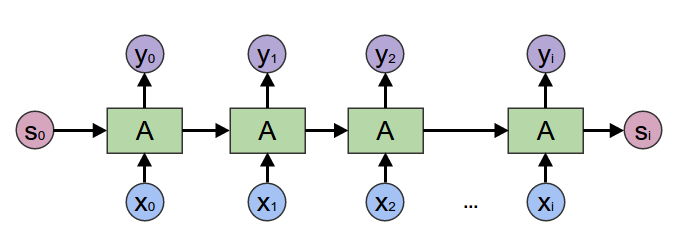
\includegraphics{/img/entries/functional-models/RNN-general.png}
\caption{Christopher Olah's RNN Unrolling Diagram}
\end{figure}

If we look at each one of those individual boxes, they all have two inputs
(normal input, and previous state) and two outputs (normal output, new state).

``Unrolling'' a stateful model means taking a model that takes in an \texttt{X}
and producing a \texttt{Y} and turning it into a model that takes an
\texttt{{[}X{]}} and produces a \texttt{{[}Y{]}}, by feeding it each of the
\texttt{X}s one after the other, propagating the state, and collecting all of
the \texttt{Y} responses.

The ``type'' of this sounds like:

\begin{Shaded}
\begin{Highlighting}[]
\OtherTok{unroll ::} \DataTypeTok{Model}\NormalTok{ p s a b }\OtherTok{->} \DataTypeTok{Model}\NormalTok{ p s [a] [b]}
\end{Highlighting}
\end{Shaded}

In writing this out as a type, we also note that the \texttt{p} parameter type
is the same, and the \texttt{s} state type is the same. (Aren't types nice? They
force you to have to think about subtle things like this) If you're familiar
with category theory, this looks a little bit like a sort of ``fmap'' under a
\texttt{Model\ p\ s} category -- it takes a (stateful and backpropagatable)
\texttt{a\ -\textgreater{}\ b} and turns it into an
\texttt{{[}a{]}\ -\textgreater{}\ {[}b{]}}.

Olah's post suggests that this is a \texttt{mapAccum}, in functional programming
parlance. And, surely enough, we can actually write this as a
\texttt{mapAccumL}.

\texttt{mapAccumL} is sort of like a combination of a \texttt{foldl} and a
\texttt{map}:

\begin{Shaded}
\begin{Highlighting}[]
\NormalTok{mapAccumL}
\OtherTok{    ::} \DataTypeTok{Traversable}\NormalTok{ t}
    \OtherTok{=>}\NormalTok{ (a }\OtherTok{->}\NormalTok{ b }\OtherTok{->}\NormalTok{ (a, c))}
    \OtherTok{->}\NormalTok{ a}
    \OtherTok{->}\NormalTok{ t b}
    \OtherTok{->}\NormalTok{ (a, t c)}
\end{Highlighting}
\end{Shaded}

Compare to \texttt{foldl}:

\begin{Shaded}
\begin{Highlighting}[]
\NormalTok{foldl}
\OtherTok{    ::} \DataTypeTok{Foldable}\NormalTok{ t}
    \OtherTok{=>}\NormalTok{ (a }\OtherTok{->}\NormalTok{ b }\OtherTok{->}\NormalTok{ a)}
    \OtherTok{->}\NormalTok{ a}
    \OtherTok{->}\NormalTok{ t b}
    \OtherTok{->}\NormalTok{ a}
\end{Highlighting}
\end{Shaded}

You can see that \texttt{mapAccumL} is just \texttt{foldl}, except the folding
function emits an extra \texttt{c} for every item, so \texttt{mapAccumL} can
return a new \texttt{t\ c} with all of the emitted \texttt{c}s.

The \emph{backprop} library has a ``lifted'' \texttt{mapAccumL} in in the
\emph{\href{http://hackage.haskell.org/package/backprop/docs/Prelude-Backprop.html}{Prelude.Backprop}}
module that we can use:

\begin{Shaded}
\begin{Highlighting}[]
\NormalTok{Prelude.Backprop.mapAccumL}
\OtherTok{    ::} \DataTypeTok{Traversable}\NormalTok{ t}
    \OtherTok{=>}\NormalTok{ (}\DataTypeTok{BVar}\NormalTok{ z a }\OtherTok{->} \DataTypeTok{BVar}\NormalTok{ z b }\OtherTok{->}\NormalTok{ (}\DataTypeTok{BVar}\NormalTok{ z a, }\DataTypeTok{BVar}\NormalTok{ z c))}
    \OtherTok{->} \DataTypeTok{BVar}\NormalTok{ z a}
    \OtherTok{->} \DataTypeTok{BVar}\NormalTok{ z (t b)}
    \OtherTok{->}\NormalTok{ (}\DataTypeTok{BVar}\NormalTok{ z a, }\DataTypeTok{BVar}\NormalTok{ z (t c))}
\end{Highlighting}
\end{Shaded}

It is lifted to work with \texttt{BVar}s of the items instead of directly on the
items. With that, we can write \texttt{unroll}, which is just a thin wrapper
over \texttt{mapAccumL}:

\begin{Shaded}
\begin{Highlighting}[]
\CommentTok{-- source: https://github.com/mstksg/inCode/tree/master/code-samples/functional-models/model.hs#L224-L232}

\NormalTok{unroll}
\OtherTok{    ::}\NormalTok{ (}\DataTypeTok{Traversable}\NormalTok{ t, }\DataTypeTok{Backprop}\NormalTok{ a, }\DataTypeTok{Backprop}\NormalTok{ b, }\DataTypeTok{Backprop}\NormalTok{ (t b))}
    \OtherTok{=>} \DataTypeTok{ModelS}\NormalTok{ p s    a     b}
    \OtherTok{->} \DataTypeTok{ModelS}\NormalTok{ p s (t a) (t b)}
\NormalTok{unroll f p xs s0 }\FunctionTok{=}\NormalTok{ swap }\FunctionTok{$}\NormalTok{ B.mapAccumL f' s0 xs}
  \KeywordTok{where}
    \CommentTok{-- we have to re-arrange the order of arguments and tuple a bit to}
    \CommentTok{-- match what `mapAccumL` expects}
\NormalTok{    f' s x }\FunctionTok{=}\NormalTok{ swap (f p x s)}
\end{Highlighting}
\end{Shaded}

This reveals that \texttt{unroll} from the machine learning is really
\emph{just} \texttt{mapAccumL} from functional programming.

We can also tweak \texttt{unroll}'s result a bit to get a version of
\texttt{unroll} that shows only the ``final'' result:

\begin{Shaded}
\begin{Highlighting}[]
\CommentTok{-- source: https://github.com/mstksg/inCode/tree/master/code-samples/functional-models/model.hs#L234-L238}

\NormalTok{unrollLast}
\OtherTok{    ::}\NormalTok{ (}\DataTypeTok{Traversable}\NormalTok{ t, }\DataTypeTok{Backprop}\NormalTok{ a, }\DataTypeTok{Backprop}\NormalTok{ b, }\DataTypeTok{Backprop}\NormalTok{ (t b))}
    \OtherTok{=>} \DataTypeTok{ModelS}\NormalTok{ p s    a  b}
    \OtherTok{->} \DataTypeTok{ModelS}\NormalTok{ p s (t a) b}
\NormalTok{unrollLast f }\FunctionTok{=}\NormalTok{ mapS (last }\FunctionTok{.}\NormalTok{ B.toList) (unroll f)}
\end{Highlighting}
\end{Shaded}

To see how this applies to our \texttt{threeLayer}:

\begin{Shaded}
\begin{Highlighting}[]
\OtherTok{threeLayers            ::} \DataTypeTok{ModelS}\NormalTok{ _ _ (}\DataTypeTok{R} \DecValTok{40}\NormalTok{) (}\DataTypeTok{R} \DecValTok{5}\NormalTok{)}
\NormalTok{unroll}\OtherTok{ threeLayers     ::} \DataTypeTok{ModelS}\NormalTok{ _ _ [}\DataTypeTok{R} \DecValTok{40}\NormalTok{] [}\DataTypeTok{R} \DecValTok{5}\NormalTok{]}
\NormalTok{unrollLast}\OtherTok{ threeLayers ::} \DataTypeTok{ModelS}\NormalTok{ _ _ [}\DataTypeTok{R} \DecValTok{40}\NormalTok{] (}\DataTypeTok{R} \DecValTok{5}\NormalTok{)}
\end{Highlighting}
\end{Shaded}

Aren't statically typed languages great?

(Note here we can use \texttt{\_} as a type variable wildcard when we don't care
about the type enough to write it)

\hypertarget{state-be-gone}{%
\subsection{State-be-gone}\label{state-be-gone}}

Did you enjoy the detour through stateful time series models?

Good! Because the whole point of it was to talk about how we can \emph{get rid
of state} and bring us back to our original models!

You knew this had to come, because all of our methods for ``training'' these
models and learn these parameters involves non-stateful models. Let's see now
how we can turn our functional stateful models into functional non-stateful
models!

One way is to \emph{fix the initial state and throw away the resulting one}.
This is very common in machine learning contexts, where many people simply fix
the initial state to be a zero vector.

\begin{Shaded}
\begin{Highlighting}[]
\CommentTok{-- source: https://github.com/mstksg/inCode/tree/master/code-samples/functional-models/model.hs#L240-L250}

\NormalTok{fixState}
\OtherTok{    ::}\NormalTok{ s}
    \OtherTok{->} \DataTypeTok{ModelS}\NormalTok{ p s a b}
    \OtherTok{->} \DataTypeTok{Model}\NormalTok{  p   a b}
\NormalTok{fixState s0 f p x }\FunctionTok{=}\NormalTok{ fst }\FunctionTok{$}\NormalTok{ f p x (auto s0)}

\NormalTok{zeroState}
\OtherTok{    ::} \DataTypeTok{Num}\NormalTok{ s}
    \OtherTok{=>} \DataTypeTok{ModelS}\NormalTok{ p s a b}
    \OtherTok{->} \DataTypeTok{Model}\NormalTok{  p   a b}
\NormalTok{zeroState }\FunctionTok{=}\NormalTok{ fixState }\DecValTok{0}
\end{Highlighting}
\end{Shaded}

We use \texttt{auto\ ::\ a\ -\textgreater{}\ BVar\ z\ a} again to introduce a
\texttt{BVar} of our initial state, but to indicate that we don't expect to
track its gradient. \texttt{zeroState} is a nice utility combinator for a common
pattern.

Another way is to \emph{treat the initial state as a trainable parameter} (and
also throw away the final state). This is not done as often, but is still common
enough to be mentioned often. And, it's just as straightforward!

\begin{Shaded}
\begin{Highlighting}[]
\CommentTok{-- source: https://github.com/mstksg/inCode/tree/master/code-samples/functional-models/model.hs#L252-L259}

\NormalTok{trainState}
\OtherTok{    ::}\NormalTok{ (}\DataTypeTok{Backprop}\NormalTok{ p, }\DataTypeTok{Backprop}\NormalTok{ s)}
    \OtherTok{=>} \DataTypeTok{ModelS}\NormalTok{  p    s  a b}
    \OtherTok{->} \DataTypeTok{Model}\NormalTok{  (p }\FunctionTok{:&}\NormalTok{ s) a b}
\NormalTok{trainState f ps x }\FunctionTok{=}\NormalTok{ fst }\FunctionTok{$}\NormalTok{ f p x s}
  \KeywordTok{where}
\NormalTok{    p }\FunctionTok{=}\NormalTok{ ps }\FunctionTok{^^.}\NormalTok{ t1}
\NormalTok{    s }\FunctionTok{=}\NormalTok{ ps }\FunctionTok{^^.}\NormalTok{ t2}
\end{Highlighting}
\end{Shaded}

\texttt{trainState} will take a model with trainable parameter \texttt{p} and
state \texttt{s}, and turn it into a model with trainable parameter
\texttt{p\ :\&\ s}, where the \texttt{s} is the (trainable) initial state.

We can now \emph{train} our recurrent/stateful models, by \textbf{unrolling and
de-stating}:

\begin{Shaded}
\begin{Highlighting}[]
\OtherTok{threeLayers                        ::} \DataTypeTok{ModelS}\NormalTok{ _ _ (}\DataTypeTok{R} \DecValTok{40}\NormalTok{) (}\DataTypeTok{R} \DecValTok{5}\NormalTok{)}
\NormalTok{unrollLast}\OtherTok{ threeLayers             ::} \DataTypeTok{ModelS}\NormalTok{ _ _ [}\DataTypeTok{R} \DecValTok{40}\NormalTok{] (}\DataTypeTok{R} \DecValTok{5}\NormalTok{)}
\NormalTok{zeroState (unrollLast threeLayers)}\OtherTok{ ::} \DataTypeTok{Model}\NormalTok{  _   [}\DataTypeTok{R} \DecValTok{40}\NormalTok{] (}\DataTypeTok{R} \DecValTok{5}\NormalTok{)}
\end{Highlighting}
\end{Shaded}

\texttt{zeroState\ (unrollLast\ threeLayers)} is now a normal stateless (and
trainable) model. It takes a list of inputs \texttt{R\ 40}s and produces the
``final output'' \texttt{R\ 5}. We can now train this by feeding it with
\texttt{({[}R\ 40{]},\ R\ 5)} pairs: give a history and an expected next output.

\hypertarget{show-me-a-sine}{%
\subsection{Show me a Sine}\label{show-me-a-sine}}

Let's see if we can train a two-layer fully connected neural network with 30
hidden units, where the first layer is fully recurrent, to learn how to model a
sine wave:

\begin{Shaded}
\begin{Highlighting}[]
\CommentTok{-- sine signal with period 25}
\NormalTok{ghci}\FunctionTok{>}\NormalTok{ series }\FunctionTok{=}\NormalTok{ [ sin (}\DecValTok{2} \FunctionTok{*}\NormalTok{ pi }\FunctionTok{*}\NormalTok{ t }\FunctionTok{/} \DecValTok{25}\NormalTok{) }\FunctionTok{|}\NormalTok{ t }\OtherTok{<-}\NormalTok{ [}\DecValTok{0}\FunctionTok{..}\NormalTok{]              ]}

\CommentTok{-- chunks of runs and "next results"}
\NormalTok{ghci}\FunctionTok{>}\NormalTok{ samps  }\FunctionTok{=}\NormalTok{ [ (init c, last c)      }\FunctionTok{|}\NormalTok{ c }\OtherTok{<-}\NormalTok{ chunksOf }\DecValTok{19}\NormalTok{ series ]}

\CommentTok{-- first layer is RNN, second layer is normal ANN, 30 hidden units}
\NormalTok{ghci}\FunctionTok{>} \KeywordTok{let}\OtherTok{ rnn ::} \DataTypeTok{ModelS}\NormalTok{ _ _ (}\DataTypeTok{R} \DecValTok{1}\NormalTok{) (}\DataTypeTok{R} \DecValTok{1}\NormalTok{)}
\NormalTok{          rnn }\FunctionTok{=}\NormalTok{ feedForward }\FunctionTok{@}\DecValTok{30} \FunctionTok{@}\DecValTok{1} \FunctionTok{<*~}\NormalTok{ mapS logistic (fcrnn }\FunctionTok{@}\DecValTok{1} \FunctionTok{@}\DecValTok{30}\NormalTok{)}

\NormalTok{ghci}\FunctionTok{>}\NormalTok{ trained }\OtherTok{<-}\NormalTok{ trainModelIO (zeroState (unrollLast rnn)) }\FunctionTok{$}\NormalTok{ take }\DecValTok{10000}\NormalTok{ samps}
\end{Highlighting}
\end{Shaded}

Trained! \texttt{trained} is now the weight and bias matrices and vectors that
will simulate a sine wave of period 25.

We can run this model iteratively upon itself to test it; if we plot the
results, we can visually inspect it to see if it has learned things properly.

Let's define some helper functions to test our model. First, a function
\texttt{prime} that takes a stateful model and gives a ``warmed-up'' state by
running it over a list of inputs. This serves to essentially initialize the
memory of the model.

\begin{Shaded}
\begin{Highlighting}[]
\CommentTok{-- source: https://github.com/mstksg/inCode/tree/master/code-samples/functional-models/model.hs#L261-L268}

\NormalTok{prime}
\OtherTok{    ::} \DataTypeTok{Foldable}\NormalTok{ t}
    \OtherTok{=>} \DataTypeTok{ModelS}\NormalTok{ p s a b     }\CommentTok{-- ^ model}
    \OtherTok{->}\NormalTok{ p                  }\CommentTok{-- ^ parameterization}
    \OtherTok{->}\NormalTok{ s                  }\CommentTok{-- ^ initial state}
    \OtherTok{->}\NormalTok{ t a                }\CommentTok{-- ^ priming input}
    \OtherTok{->}\NormalTok{ s                  }\CommentTok{-- ^ primed state}
\NormalTok{prime f p }\FunctionTok{=}\NormalTok{ foldl' }\FunctionTok{$}\NormalTok{ evalBP2 (\textbackslash{}s x }\OtherTok{->}\NormalTok{ snd }\FunctionTok{$}\NormalTok{ f (auto p) x s)}
\end{Highlighting}
\end{Shaded}

Then a function \texttt{feedback} that iterates a stateful model over and over
again by feeding its previous output as its next input:

\begin{Shaded}
\begin{Highlighting}[]
\CommentTok{-- source: https://github.com/mstksg/inCode/tree/master/code-samples/functional-models/model.hs#L270-L281}

\NormalTok{feedback}
\OtherTok{    ::}\NormalTok{ (}\DataTypeTok{Backprop}\NormalTok{ a, }\DataTypeTok{Backprop}\NormalTok{ s)}
    \OtherTok{=>} \DataTypeTok{ModelS}\NormalTok{ p s a a     }\CommentTok{-- ^ model}
    \OtherTok{->}\NormalTok{ p                  }\CommentTok{-- ^ parameterization}
    \OtherTok{->}\NormalTok{ s                  }\CommentTok{-- ^ initial state}
    \OtherTok{->}\NormalTok{ a                  }\CommentTok{-- ^ initial input}
    \OtherTok{->}\NormalTok{ [a]                }\CommentTok{-- ^ inifinite feedback loop}
\NormalTok{feedback f p s0 x0 }\FunctionTok{=}\NormalTok{ unfoldr go (x0, s0)}
  \KeywordTok{where}
\NormalTok{    go (x, s) }\FunctionTok{=} \DataTypeTok{Just}\NormalTok{ (x, (y, s'))}
      \KeywordTok{where}
\NormalTok{        (y, s') }\FunctionTok{=}\NormalTok{ evalBP (uncurry }\DataTypeTok{T2} \FunctionTok{.}\NormalTok{ f (auto p) (auto x)) s}
\end{Highlighting}
\end{Shaded}

Now let's prime our trained model over the first 19 items in our sine wave and
start it running in feedback mode on the 20th item!

\begin{Shaded}
\begin{Highlighting}[]
\NormalTok{ghci}\FunctionTok{>} \KeywordTok{let}\NormalTok{ primed }\FunctionTok{=}\NormalTok{ prime    rnn trained }\DecValTok{0}\NormalTok{      (take }\DecValTok{19}\NormalTok{ series)}
\NormalTok{ghci}\FunctionTok{>} \KeywordTok{let}\NormalTok{ output }\FunctionTok{=}\NormalTok{ feedback rnn trained primed (series }\FunctionTok{!!} \DecValTok{19}\NormalTok{)}
\NormalTok{ghci}\FunctionTok{>}\NormalTok{ mapM_ print }\FunctionTok{$}\NormalTok{ take }\DecValTok{200}\NormalTok{ output}
\NormalTok{(}\FunctionTok{-}\FloatTok{0.9980267284282716}\OtherTok{ ::} \DataTypeTok{R} \DecValTok{1}\NormalTok{)}
\NormalTok{(}\FunctionTok{-}\FloatTok{0.9530599469923343}\OtherTok{ ::} \DataTypeTok{R} \DecValTok{1}\NormalTok{)}
\NormalTok{(}\FunctionTok{-}\FloatTok{0.855333250123637}\OtherTok{ ::} \DataTypeTok{R} \DecValTok{1}\NormalTok{)}
\NormalTok{(}\FunctionTok{-}\FloatTok{0.7138776465246676}\OtherTok{ ::} \DataTypeTok{R} \DecValTok{1}\NormalTok{)}
\NormalTok{(}\FunctionTok{-}\FloatTok{0.5359655931506458}\OtherTok{ ::} \DataTypeTok{R} \DecValTok{1}\NormalTok{)}
\CommentTok{-- ...}
\end{Highlighting}
\end{Shaded}

Plotting the result against the ``actual'' sine wave of period 25, we see that
it approximates the process decently well, with a consistent period:

\begin{figure}
\centering
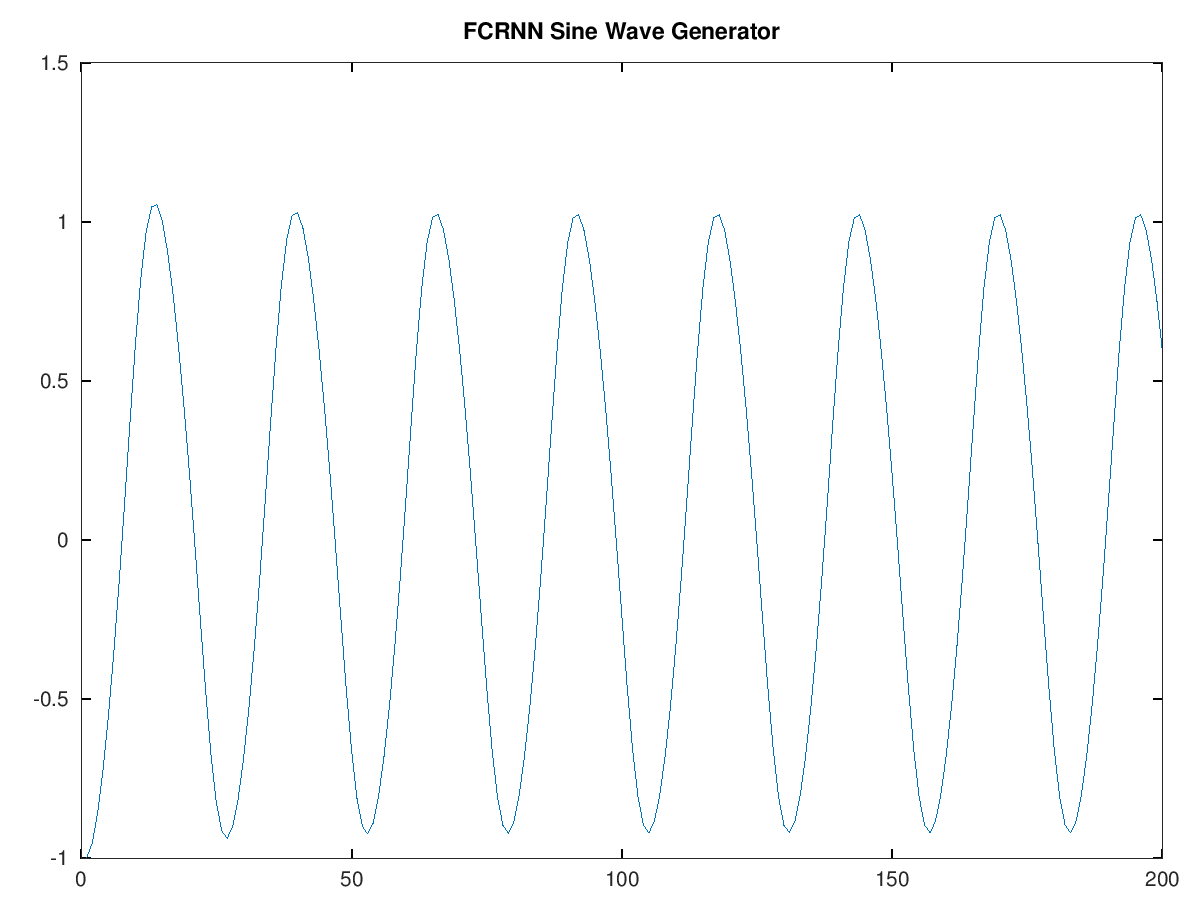
\includegraphics{/img/entries/functional-models/rnnsin.png}
\caption{FCRNN Sine Wave}
\end{figure}

Not perfect, but still looks a bit ``unreasonably effective'', eh?

For kicks, let's see if we can do any better with the simpler AR(2) model from
before. Applying all we just used to \texttt{ar2}, we see:

\begin{Shaded}
\begin{Highlighting}[]
\OtherTok{ar2                        ::} \DataTypeTok{ModelS}\NormalTok{ _ _  }\DataTypeTok{Double}  \DataTypeTok{Double}
\NormalTok{unrollLast}\OtherTok{ ar2             ::} \DataTypeTok{ModelS}\NormalTok{ _ _ [}\DataTypeTok{Double}\NormalTok{] }\DataTypeTok{Double}
\NormalTok{zeroState (unrollLast ar2)}\OtherTok{ ::} \DataTypeTok{Model}\NormalTok{  _   [}\DataTypeTok{Double}\NormalTok{] }\DataTypeTok{Double}
\end{Highlighting}
\end{Shaded}

\texttt{zeroState\ (unrollLast\ ar2)} is now a trainable stateless model. Will
it model a sine wave?

\begin{Shaded}
\begin{Highlighting}[]
\NormalTok{ghci}\FunctionTok{>}\NormalTok{ trained }\OtherTok{<-}\NormalTok{ trainModelIO (zeroState (unrollLast ar2)) }\FunctionTok{$}\NormalTok{ take }\DecValTok{10000}\NormalTok{ samps}
\NormalTok{ghci}\FunctionTok{>} \KeywordTok{let}\NormalTok{ primed }\FunctionTok{=}\NormalTok{ prime    rnn trained }\DecValTok{0}\NormalTok{      (take }\DecValTok{19}\NormalTok{ series)}
\NormalTok{ghci}\FunctionTok{>} \KeywordTok{let}\NormalTok{ output }\FunctionTok{=}\NormalTok{ feedback rnn trained primed (series }\FunctionTok{!!} \DecValTok{19}\NormalTok{)}
\NormalTok{ghci}\FunctionTok{>}\NormalTok{ mapM_ print }\FunctionTok{$}\NormalTok{ take }\DecValTok{200}\NormalTok{ output}
\NormalTok{(}\FunctionTok{-}\FloatTok{0.9980267284282716}\OtherTok{ ::} \DataTypeTok{R} \DecValTok{1}\NormalTok{)}
\NormalTok{(}\FunctionTok{-}\FloatTok{0.9530599469923343}\OtherTok{ ::} \DataTypeTok{R} \DecValTok{1}\NormalTok{)}
\NormalTok{(}\FunctionTok{-}\FloatTok{0.855333250123637}\OtherTok{ ::} \DataTypeTok{R} \DecValTok{1}\NormalTok{)}
\NormalTok{(}\FunctionTok{-}\FloatTok{0.7138776465246676}\OtherTok{ ::} \DataTypeTok{R} \DecValTok{1}\NormalTok{)}
\NormalTok{(}\FunctionTok{-}\FloatTok{0.5359655931506458}\OtherTok{ ::} \DataTypeTok{R} \DecValTok{1}\NormalTok{)}
\CommentTok{-- ...}
\end{Highlighting}
\end{Shaded}

We can plot the result and see that it more or less perfectly models the sine
wave of period 25:

\begin{figure}
\centering
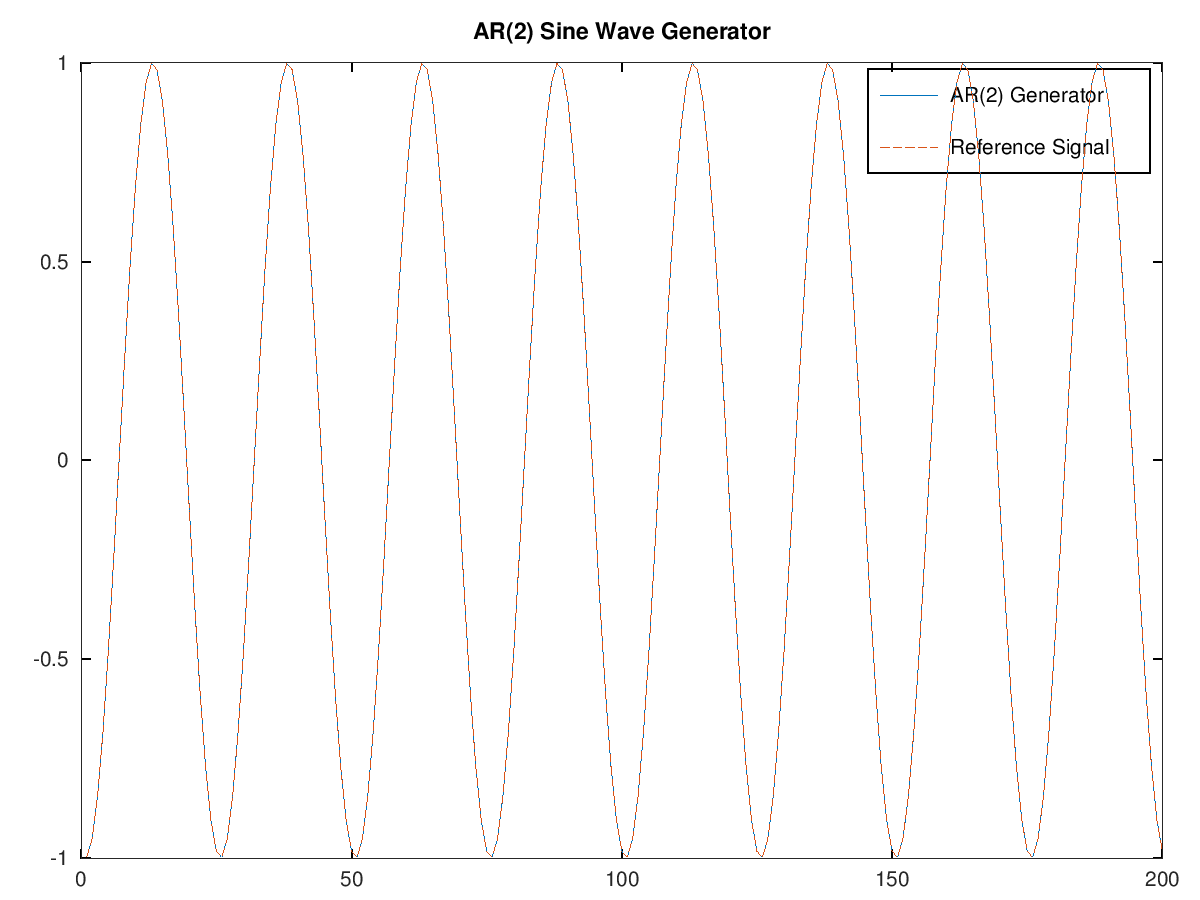
\includegraphics{/img/entries/functional-models/ar2sin.png}
\caption{AR(2) Sine Wave}
\end{figure}

You can't even visually see the difference!

We can peek inside the parameterization of our learned AR(2):

\begin{Shaded}
\begin{Highlighting}[]
\NormalTok{ghci}\FunctionTok{>}\NormalTok{ trained}
\FunctionTok{-}\FloatTok{2.4013298985824788e-12} \FunctionTok{:&}\NormalTok{ (}\FloatTok{1.937166322256747} \FunctionTok{:&} \FunctionTok{-}\FloatTok{0.9999999999997953}\NormalTok{)}
\CommentTok{-- approximately}
\FloatTok{0.00} \FunctionTok{:&}\NormalTok{ (}\FloatTok{1.94} \FunctionTok{:&} \FunctionTok{-}\FloatTok{1.00}\NormalTok{)}
\end{Highlighting}
\end{Shaded}

Meaning that the gradient descent has concluded that our AR(2) model is:

{[} y\_t = 0 + 1.94 y\_\{t - 1\} - y\_\{t -
2\}{]}(https://latex.codecogs.com/png.latex?\%0Ay\_t\%20\%3D\%200\%20\%2B\%201.94\%20y\_\%7Bt\%20-\%201\%7D\%20-\%20y\_\%7Bt\%20-\%202\%7D\%0A
" y\_t = 0 + 1.94 y\_\{t - 1\} - y\_\{t - 2\} ``)

In this toy situation, the AR(2) appears to do much better than our RNN model,
but we have to give the RNN a break --- all of the information has to be
``squished'' into essentially 30 bits, which might impact the model's accuracy.

\hypertarget{functions-all-the-way-down}{%
\section{Functions all the way down}\label{functions-all-the-way-down}}

Again, it is very easy to look at something like

\begin{Shaded}
\begin{Highlighting}[]
\NormalTok{feedForward }\FunctionTok{@}\DecValTok{30} \FunctionTok{@}\DecValTok{1} \FunctionTok{<*~}\NormalTok{ mapS logistic (fcrnn }\FunctionTok{@}\DecValTok{1} \FunctionTok{@}\DecValTok{30}\NormalTok{)}
\end{Highlighting}
\end{Shaded}

and write it off as some abstract API of opaque data types. Some sort of object
keeps track of state, and the object has some nice abstracted
interface\ldots{}right?

But, nope, again, it is all just normal functions that we wrote using normal
function composition. We define our model as a \emph{function}, and the backprop
library turns that function into a trainable model.

\hypertarget{combinator-fun}{%
\subsection{Combinator Fun}\label{combinator-fun}}

I really like how we have pretty much free reign over how we can combine and
manipulate our models, since they are just functions.

\hypertarget{recurrence-is-a-combinator}{%
\subsubsection{Recurrence is a Combinator}\label{recurrence-is-a-combinator}}

Here's one example of how the freedom that ``normal functions'' gives you can
help reveal insight. I stumbled upon an interesting way of defining recurrent
neural networks --- a lot of times, a ``recurrent neural network'' really just
means that some function of the \emph{previous} output is used as an ``extra
input''.

This sounds like we can really write a recurrent model as a ``normal'' model,
and then use a combinator to feed it back into itself.

To say in types:

\begin{Shaded}
\begin{Highlighting}[]
\NormalTok{recurrently}
\OtherTok{    ::} \DataTypeTok{Model}\NormalTok{  p   (a }\FunctionTok{:&}\NormalTok{ b) b}
    \OtherTok{->} \DataTypeTok{ModelS}\NormalTok{ p b  a       b}
\end{Highlighting}
\end{Shaded}

A ``normal, non-stateful model'' taking an \texttt{a\ :\&\ b} and returning a
\texttt{b} can really be turned into a stateful model with state \texttt{b} (the
\emph{previous output}) and only taking in an \texttt{a} input.

This sort of combinator is a joy to write in Haskell because it's a ``follow the
types'' kinda deal --- you set up the function, and the compiler pretty much
writes it for you, because the types guide the entire implementation:

\begin{Shaded}
\begin{Highlighting}[]
\CommentTok{-- source: https://github.com/mstksg/inCode/tree/master/code-samples/functional-models/model.hs#L317-L323}

\NormalTok{recurrently}
\OtherTok{    ::}\NormalTok{ (}\DataTypeTok{Backprop}\NormalTok{ a, }\DataTypeTok{Backprop}\NormalTok{ b)}
    \OtherTok{=>} \DataTypeTok{Model}\NormalTok{  p   (a }\FunctionTok{:&}\NormalTok{ b) b}
    \OtherTok{->} \DataTypeTok{ModelS}\NormalTok{ p b  a       b}
\NormalTok{recurrently f p x yLast }\FunctionTok{=}\NormalTok{ (y, y)}
  \KeywordTok{where}
\NormalTok{    y }\FunctionTok{=}\NormalTok{ f p (x }\FunctionTok{#&}\NormalTok{ yLast)}
\end{Highlighting}
\end{Shaded}

In general though, it'd be nice to have \emph{some function} of the previous
output be stored as the state. We can write this combinator as well, taking the
function that transforms the previous output into the stored state:

\begin{Shaded}
\begin{Highlighting}[]
\CommentTok{-- source: https://github.com/mstksg/inCode/tree/master/code-samples/functional-models/model.hs#L325-L332}

\NormalTok{recurrentlyWith}
\OtherTok{    ::}\NormalTok{ (}\DataTypeTok{Backprop}\NormalTok{ a, }\DataTypeTok{Backprop}\NormalTok{ b)}
    \OtherTok{=>}\NormalTok{ (forall z}\FunctionTok{.} \DataTypeTok{Reifies}\NormalTok{ z }\DataTypeTok{W} \OtherTok{=>} \DataTypeTok{BVar}\NormalTok{ z c }\OtherTok{->} \DataTypeTok{BVar}\NormalTok{ z b)}
    \OtherTok{->} \DataTypeTok{Model}\NormalTok{  p   (a }\FunctionTok{:&}\NormalTok{ b) c}
    \OtherTok{->} \DataTypeTok{ModelS}\NormalTok{ p b  a       c}
\NormalTok{recurrentlyWith store f p x yLast }\FunctionTok{=}\NormalTok{ (y, store y)}
  \KeywordTok{where}
\NormalTok{    y }\FunctionTok{=}\NormalTok{ f p (x }\FunctionTok{#&}\NormalTok{ yLast)}
\end{Highlighting}
\end{Shaded}

Again, once we figure out the \emph{type} our combinator has\ldots{}the function
writes itself. The joys of Haskell!

\texttt{recurrentlyWith} takes a \texttt{c\ -\textgreater{}\ b} function and
turns a pure model taking an \texttt{a\ :\&\ b} into a stateful model with state
\texttt{b} taking in an \texttt{a}. The \texttt{c\ -\textgreater{}\ b} tells you
how to turn the previous output into the new state.

To me, \texttt{recurrentlyWith} captures the ``essence'' of what a recurrent
model or recurrent neural network is --- the network is allowed to ``see'' its
previous output.

And the piece de resistance --- we can use this to define a fully connected
recurrent neural network layer as simply a recurrent version of a normal fully
connected feed-forward layer.

We can redefine a pre-mapped version of \texttt{feedForward} which takes a tuple
of two vectors and concatenates them before doing anything:

\begin{Shaded}
\begin{Highlighting}[]
\CommentTok{-- | Concatenate two vectors}
\OtherTok{(#)          ::} \DataTypeTok{BVar}\NormalTok{ s (}\DataTypeTok{R}\NormalTok{ i) }\OtherTok{->} \DataTypeTok{BVar}\NormalTok{ s (}\DataTypeTok{R}\NormalTok{ o) }\OtherTok{->} \DataTypeTok{BVar}\NormalTok{ s (}\DataTypeTok{R}\NormalTok{ (i }\FunctionTok{+}\NormalTok{ o))}
\CommentTok{-- source: https://github.com/mstksg/inCode/tree/master/code-samples/functional-models/model.hs#L334-L340}

\NormalTok{ffOnSplit}
\OtherTok{    ::}\NormalTok{ forall i o}\FunctionTok{.}\NormalTok{ (}\DataTypeTok{KnownNat}\NormalTok{ i, }\DataTypeTok{KnownNat}\NormalTok{ o)}
    \OtherTok{=>} \DataTypeTok{Model}\NormalTok{ _ (}\DataTypeTok{R}\NormalTok{ i }\FunctionTok{:&} \DataTypeTok{R}\NormalTok{ o) (}\DataTypeTok{R}\NormalTok{ o)}
\NormalTok{ffOnSplit p rIrO }\FunctionTok{=}\NormalTok{ feedForward }\FunctionTok{@}\NormalTok{(i }\FunctionTok{+}\NormalTok{ o) p (rI }\FunctionTok{#}\NormalTok{ rO)}
  \KeywordTok{where}
\NormalTok{    rI }\FunctionTok{=}\NormalTok{ rIrO }\FunctionTok{^^.}\NormalTok{ t1}
\NormalTok{    rO }\FunctionTok{=}\NormalTok{ rIrO }\FunctionTok{^^.}\NormalTok{ t2}
\end{Highlighting}
\end{Shaded}

\texttt{ffOnSplit} is a feed-forward layer taking an \texttt{R\ (i\ +\ o)},
except we pre-map it to take a tuple \texttt{R\ i\ :\&\ R\ o} instead.

Now our fully connected recurrent layer is just
\texttt{recurrentlyWith\ logistic\ ffOnSplit}:

\begin{Shaded}
\begin{Highlighting}[]
\NormalTok{fcrnn'}
\OtherTok{    ::}\NormalTok{ (}\DataTypeTok{KnownNat}\NormalTok{ i, }\DataTypeTok{KnownNat}\NormalTok{ o)}
    \OtherTok{=>} \DataTypeTok{ModelS}\NormalTok{ _ (}\DataTypeTok{R}\NormalTok{ o) (}\DataTypeTok{R}\NormalTok{ i) (}\DataTypeTok{R}\NormalTok{ o)}
\NormalTok{fcrnn' }\FunctionTok{=}\NormalTok{ recurrentlyWith logistic ffOnSplit}
\end{Highlighting}
\end{Shaded}

Basically just a recurrent version of \texttt{feedForward}! If we abstract out
some of the manual uncurrying and pre-mapping, we get a nice functional
definition:

\begin{Shaded}
\begin{Highlighting}[]
\CommentTok{-- source: https://github.com/mstksg/inCode/tree/master/code-samples/functional-models/model.hs#L342-L345}

\NormalTok{fcrnn'}
\OtherTok{    ::}\NormalTok{ (}\DataTypeTok{KnownNat}\NormalTok{ i, }\DataTypeTok{KnownNat}\NormalTok{ o)}
    \OtherTok{=>} \DataTypeTok{ModelS}\NormalTok{ _ (}\DataTypeTok{R}\NormalTok{ o) (}\DataTypeTok{R}\NormalTok{ i) (}\DataTypeTok{R}\NormalTok{ o)}
\NormalTok{fcrnn' }\FunctionTok{=}\NormalTok{ recurrentlyWith logistic (\textbackslash{}p }\OtherTok{->}\NormalTok{ feedForward p }\FunctionTok{.}\NormalTok{ uncurryT (}\FunctionTok{#}\NormalTok{))}
\end{Highlighting}
\end{Shaded}

\hypertarget{lagging-is-a-combinator}{%
\subsubsection{Lagging is a Combinator}\label{lagging-is-a-combinator}}

Another interesting result -- we can write a ``lagged'' combinator that takes a
model expecting a vector as an input, and turn it into a stateful model taking a
\emph{single} input, and feeding the original model that input and also a
history of the \texttt{n} most recent inputs.

If that sounds confusing, let's just try to state it out using types:

\begin{Shaded}
\begin{Highlighting}[]
\OtherTok{lagged ::} \DataTypeTok{Model}\NormalTok{  p       (}\DataTypeTok{R}\NormalTok{ (n }\FunctionTok{+} \DecValTok{1}\NormalTok{)) b}
       \OtherTok{->} \DataTypeTok{ModelS}\NormalTok{ p (}\DataTypeTok{R}\NormalTok{ n) }\DataTypeTok{Double}\NormalTok{      b}
\end{Highlighting}
\end{Shaded}

The result is a \texttt{ModelS\ p\ (R\ n)\ Double\ b}; the state is the
\texttt{n} most recent inputs, and it feeds that in at every step and keeps it
updated. Let's write it using \texttt{headTail} and \texttt{\&}, which splits a
vector and adds an item to the end, respectively.

\begin{Shaded}
\begin{Highlighting}[]
\CommentTok{-- source: https://github.com/mstksg/inCode/tree/master/code-samples/functional-models/model.hs#L347-L355}

\NormalTok{lagged}
\OtherTok{    ::}\NormalTok{ (}\DataTypeTok{KnownNat}\NormalTok{ n, }\DecValTok{1} \FunctionTok{<=}\NormalTok{ n)}
    \OtherTok{=>} \DataTypeTok{Model}\NormalTok{  p       (}\DataTypeTok{R}\NormalTok{ (n }\FunctionTok{+} \DecValTok{1}\NormalTok{)) b}
    \OtherTok{->} \DataTypeTok{ModelS}\NormalTok{ p (}\DataTypeTok{R}\NormalTok{ n) }\DataTypeTok{Double}\NormalTok{      b}
\NormalTok{lagged f p x xLasts }\FunctionTok{=}\NormalTok{ (y, xLasts')}
  \KeywordTok{where}
\NormalTok{    fullLasts    }\FunctionTok{=}\NormalTok{ xLasts }\FunctionTok{&}\NormalTok{ x}
\NormalTok{    y            }\FunctionTok{=}\NormalTok{ f p fullLasts}
\NormalTok{    (_, xLasts') }\FunctionTok{=}\NormalTok{ headTail fullLasts}
\end{Highlighting}
\end{Shaded}

What can we do with this? Well\ldots{} we can write a general autoregressive
model AR(p) of \emph{any} degree, simply by lagging a fully connected ANN layer:

\begin{Shaded}
\begin{Highlighting}[]
\CommentTok{-- source: https://github.com/mstksg/inCode/tree/master/code-samples/functional-models/model.hs#L357-L359}

\OtherTok{ar ::}\NormalTok{ (}\DataTypeTok{KnownNat}\NormalTok{ n, }\DecValTok{1} \FunctionTok{<=}\NormalTok{ n)}
   \OtherTok{=>} \DataTypeTok{ModelS}\NormalTok{ _ (}\DataTypeTok{R}\NormalTok{ n) }\DataTypeTok{Double} \DataTypeTok{Double}
\NormalTok{ar }\FunctionTok{=}\NormalTok{ lagged (\textbackslash{}p }\OtherTok{->}\NormalTok{ fst }\FunctionTok{.}\NormalTok{ headTail }\FunctionTok{@}\NormalTok{_ }\FunctionTok{@}\DecValTok{1} \FunctionTok{.}\NormalTok{ feedForward p)}
\end{Highlighting}
\end{Shaded}

(using \texttt{fst\ .\ headTail} to extract the first \texttt{Double} from an
\texttt{R\ 1})

And that's it! Our original AR(2) \texttt{ar2} is just \texttt{ar\ @2} \ldots{}
and we can write can write an AR(10) model by just using \texttt{ar\ @10}, and
AR(20) model with \texttt{ar\ @20}, etc.

\begin{Shaded}
\begin{Highlighting}[]
\CommentTok{-- source: https://github.com/mstksg/inCode/tree/master/code-samples/functional-models/model.hs#L361-L362}

\OtherTok{ar2' ::} \DataTypeTok{ModelS}\NormalTok{ _ (}\DataTypeTok{R} \DecValTok{2}\NormalTok{) }\DataTypeTok{Double} \DataTypeTok{Double}
\NormalTok{ar2' }\FunctionTok{=}\NormalTok{ ar }\FunctionTok{@}\DecValTok{2}
\end{Highlighting}
\end{Shaded}

Who would have thought that an autoregressive model is just a fully connected
neural network layer with lag?

Take a fully connected ANN layer and add recurrence --- you get a fully
connected RNN layer. Take a fully connected ANN layer and add lag --- you get an
autoregressive model from statistics!

There are many more such combinators possible! Combinators like
\texttt{recurrentlyWith} and \texttt{lagged} just scratch the surface. Best of
all, they help reveal to us that seemingly exotic things really are just simple
applications of combinators from other basic things.

\begin{center}\rule{0.5\linewidth}{\linethickness}\end{center}

\textbf{Aside: Unified Representation}

This is a small aside for those familiar with Haskell techniques like DataKinds
and dependent types!

One ugly thing you might have noticed was that we had to give different
``types'' for both our \texttt{Model} and \texttt{ModelS}, so we cannot re-use
useful functions on both. For example, \texttt{mapS} only works on
\texttt{ModelS}, but not \texttt{Model}. \texttt{(\textless{}\textasciitilde{})}
only works on \texttt{Model}s, \texttt{(\textless{}*\textasciitilde{}*)} only
works on two \texttt{ModelS}s, and we had to define a different combinator
\texttt{(\textless{}*\textasciitilde{})}.

This is not a fundamental limitation! With \emph{DataKinds} and dependent types
we can unify these both under a common type. If we had:

\begin{Shaded}
\begin{Highlighting}[]
\KeywordTok{type} \DataTypeTok{Model}\NormalTok{ (}\OtherTok{p ::} \DataTypeTok{Type}\NormalTok{) (}\OtherTok{a ::} \DataTypeTok{Type}\NormalTok{) (}\OtherTok{b ::} \DataTypeTok{Type}\NormalTok{) }\FunctionTok{=}
\NormalTok{       forall z}\FunctionTok{.} \DataTypeTok{Reifies}\NormalTok{ z }\DataTypeTok{W}
    \OtherTok{=>} \DataTypeTok{BVar}\NormalTok{ z p}
    \OtherTok{->} \DataTypeTok{BVar}\NormalTok{ z a}
    \OtherTok{->} \DataTypeTok{BVar}\NormalTok{ z b}

\KeywordTok{type} \DataTypeTok{ModelS}\NormalTok{ (}\OtherTok{p ::} \DataTypeTok{Type}\NormalTok{) (}\OtherTok{s ::} \DataTypeTok{Type}\NormalTok{) (}\OtherTok{a ::} \DataTypeTok{Type}\NormalTok{) (}\OtherTok{b ::} \DataTypeTok{Type}\NormalTok{) }\FunctionTok{=}
\NormalTok{       forall z}\FunctionTok{.} \DataTypeTok{Reifies}\NormalTok{ z }\DataTypeTok{W}
    \OtherTok{=>} \DataTypeTok{BVar}\NormalTok{ z p}
    \OtherTok{->} \DataTypeTok{BVar}\NormalTok{ z a}
    \OtherTok{->} \DataTypeTok{BVar}\NormalTok{ z s}
    \OtherTok{->}\NormalTok{ (}\DataTypeTok{BVar}\NormalTok{ z b, }\DataTypeTok{BVar}\NormalTok{ z s)}
\end{Highlighting}
\end{Shaded}

We can unify them by making \texttt{s} be optional, a \texttt{Maybe\ Type}, and
using the \texttt{Option} type from
\emph{\href{https://hackage.haskell.org/package/type-combinators/docs/Data-Type-Option.html}{Data.Type.Option}},
from the
\emph{\href{https://hackage.haskell.org/package/type-combinators}{type-combinators}}
package:

\begin{Shaded}
\begin{Highlighting}[]
\KeywordTok{type} \DataTypeTok{Model'}\NormalTok{ (}\OtherTok{p ::} \DataTypeTok{Type}\NormalTok{) (}\OtherTok{s ::} \DataTypeTok{Maybe} \DataTypeTok{Type}\NormalTok{) (}\OtherTok{a ::} \DataTypeTok{Type}\NormalTok{) (}\OtherTok{b ::} \DataTypeTok{Type}\NormalTok{) }\FunctionTok{=}
\NormalTok{       forall z}\FunctionTok{.} \DataTypeTok{Reifies}\NormalTok{ z }\DataTypeTok{W}
    \OtherTok{=>} \DataTypeTok{BVar}\NormalTok{ z p}
    \OtherTok{->} \DataTypeTok{BVar}\NormalTok{ z a}
    \OtherTok{->} \DataTypeTok{Option}\NormalTok{ (}\DataTypeTok{BVar}\NormalTok{ z) s}
    \OtherTok{->}\NormalTok{ (}\DataTypeTok{BVar}\NormalTok{ z b, }\DataTypeTok{Option}\NormalTok{ (}\DataTypeTok{BVar}\NormalTok{ z) s)}
\end{Highlighting}
\end{Shaded}

\texttt{Option\ f\ a} contains a value if \texttt{a} is
\texttt{\textquotesingle{}Just}, and does not if \texttt{a} is
\texttt{\textquotesingle{}Nothing}.

We can then re-define our previous types:

\begin{Shaded}
\begin{Highlighting}[]
\KeywordTok{type} \DataTypeTok{Model}\NormalTok{  p   }\FunctionTok{=} \DataTypeTok{Model'}\NormalTok{ p }\CharTok{'Nothing}
\KeywordTok{type} \DataTypeTok{ModelS}\NormalTok{ p s }\FunctionTok{=} \DataTypeTok{Model'}\NormalTok{ p (}\CharTok{'Just s)}
\end{Highlighting}
\end{Shaded}

And now that we have unified everything under the same type, we can write
\texttt{mapS} that takes both stateful and non-stateful models, merge
\texttt{(\textless{}\textasciitilde{})},
\texttt{(\textless{}*\textasciitilde{}*)} and
\texttt{(\textless{}*\textasciitilde{})}, etc., thanks to the power of dependent
types.

Note that dependent types and DataKind shenanigans aren't necessary for any of
this to work --- it just has the possibility to make things even more seamless
and unified!

\begin{center}\rule{0.5\linewidth}{\linethickness}\end{center}

\hypertarget{a-path-forward}{%
\section{A Path Forward}\label{a-path-forward}}

Thank you for making it to the end! I hope at this point you have been able to
gain some appreciation for differential programming in a purely functional
style, and see the sort of doors that this opens.

At this point, we don't ever ``need'' a ``neural network library'' or a ``neural
network framework''. All we really need for a good differential programming
based library is:

\begin{itemize}
\item
  A handful of small primitive models expressed as normal functions (like
  \texttt{linReg}, \texttt{fullyConnected}, \texttt{ar2}, \texttt{lstm},
  \texttt{convulotion}, etc.)
\item
  Some useful higher-order functions acting as utility combinators to common
  patterns of function composition, like \texttt{map},
  \texttt{\textless{}\textasciitilde{}}, etc., that are never \emph{required}
  but just convenient, since the functional API is already fully featured as it
  is.

  With these, models that seem seemingly very different can be defined in terms
  of simple combinator applications of other models, and that simple base models
  can be used to derive other models in surprising ways (like how a feed-forward
  layer can be turned into a recurrent layer or an autoregressive model)
\item
  A handy collection of (differentiable) \emph{loss functions}; in this library
  we only used squared error, but in other situations there might be other
  useful ones like cross-entropy.

  Loss functions can be combined with regularizing terms from parameters, if the
  regularization functions themselves are differentiable.
\item
  A handy collection of \emph{optimizers}, allowing you to take a loss function,
  a set of samples, and a model, and return the optimal parameters using
  optimizers like stochastic gradient descent, momentum, adam, etc.
\end{itemize}

That's really it, I feel! Just the models \emph{as functions}, the combinators,
and methods to evaluate and train those functions. No ``objects'' defining
layers as data (they're not data, they're functions!); just the full freedom of
expressing a model as any old function you want.\footnote{This is the basis
  behind my work-in-progress \href{https://github.com/mstksg/opto}{opto} and
  \href{https://github.com/mstksg/backprop-learn}{backprop-learn} libraries.}

A lot of things come together to make all of this work:

\begin{enumerate}
\def\labelenumi{\arabic{enumi}.}
\item
  \emph{Functional programming}, allowing us to write higher-order functions and
  combinators that take functions and return functions. This is the entire crux
  of this approach, and lets us not only draw from mathematical models directly,
  but also combine and reshape models in arbitrary ways just by using normal
  function composition and application, instead of being forced into a rigid
  compositional model.

  We were able to chain, fork, recombine models by just writing normal
  higher-order functions.

  And, through normal higher-order functions, we can see that many models are
  just ``combinator-applied'' versions of other simpler models!
\item
  \emph{Differentiable} programs, allowing us to write normal functions and have
  them be automatically differentiable for gradient descent.
\item
  \emph{Purely} functional programming. If \emph{any} of these functions were
  side-effecting and impure functions, the correspondence between functions and
  mathematical models completely falls apart. This is something we often take
  for granted when writing Haskell, but in other languages, without purity, no
  model is sound.
\item
  A \emph{strong expressive static type system} makes this all reasonable to
  work with. A strong type system tells us how we are allowed to combine outputs
  and inputs of functions, how we can combine parameters, what values parameters
  contains, what parameters a given model contains, etc.; without this
  knowledge, it would be impossible to sanely write complex programs.

  This forces us to be aware of what parameters we have, how they combine, etc.;
  this is what makes combinators like \texttt{recurrent} and \texttt{unroll} and
  \texttt{zeroState} reasonable: the \emph{compiler} is able to trace how we
  move around our parameter and state, so that we don't have to. It lets us ask
  \emph{the compiler} questions like ``what is the state, now?'' if we needed,
  or ``what is the parameter now?''.

  We sometimes even gained insight simply from thinking, in advance, what the
  types of our combinators were. And, if we can phrase our combinators in terms
  of our types, the compiler will often be able to write our entire program for
  us --- something only possible for statically typed languages.
\end{enumerate}

If you drop any one of these pieces, you are left with something very clumsy as
a result. In an imperative or object-oriented setting with inexpressive or
dynamic type system would render this approach almost infeasible. I really feel
like, after working with these types and these sorts of models, we are peering
into the future of machine learning's gradient-trainable models.

\end{document}
